\chapter{Logic and Proofs}
Logic is very easy to understand. If it is hard for you, you have a bigger problem that this chapter cannot solve. However, to save time, mathematicians created multiple notations to make their lives easier (and our lives a bit harder). This chapter is an attempt to quickly summarize those notations and acts as a reference sheet whenever you see strange logic notations.

\section{Symbols and notations}
\textbf{Propositions} are statements that could be either true or false. We use $T$ or $F$ to indicate true or false.

A proposition can be \textbf{negated}, which gives the opposite of the proposition. The negation of $p$ is:
\begin{equation} \neg p \end{equation}
\textbf{The conjunction operator} will return true if both propositions $p$  and $q$ are true; it is similar to an "and" statement. 
\begin{equation} p \land q \end{equation}

\textbf{Disjunction} is similar to an "or" statement where it only requires either one statement to be true.
\begin{equation} p \lor q \end{equation}

\textbf{Exclusive or} (XOR) will return true if either statement is true, but not both.
\begin{equation} p \oplus q \end{equation}
It is similar to $(p \lor q)\land\neg(p \land q)$.

\textbf{Implication} expresses that one thing will result in another ("if $p$ then $q$"):
\begin{equation} p \rightarrow q \end{equation}
$p$ is called the antecedent, premise, or hypothesis; $q$ is called the conclusion or consequence because it is the result of $p$. Moreover, noted that the whole statement itself can still generate $T$ or $F$ values. If we have a statement "If the store is open today ($p$), then Luka will go ($q$)". Consider the truth table, we have:
\begin{itemize}
    \item If the store opens, then Luka will go, making $p \rightarrow q$ true.
    \item If the store opens but Luka does not go, then apparently Luka's action does not depend on the store being opened.
    \item If the stores do not open but Luka still goes, the statement $p \rightarrow q$ is still true because it does not say anything about the store being closed.
    \item If the store closes and Luka stays at home, the statement is still true for a similar reason.
\end{itemize}

A \textbf{bi-conditional statement} is similar to the statement "if and only if", that is when both propositions support each other. This is similar to the equal sign, so even if both propositions are false, the bi-conditional statements still hold (because $F=F$)
\begin{equation} p \leftrightarrow q \end{equation}
The difference is that bi-conditional implies that both $p$ and $q$ are similar to each other; that is, they are either both true or both false for $p \leftrightarrow q$ is true.

\textbf{Equivalent} are propositions that are the same. There are two ways to write it and you will usually see the latter in algebra:
\begin{equation}
    p \equiv q
    \qquad
    p \Leftrightarrow q
\end{equation}

\textbf{A predicate} is a statement with variables, written with a capital letter and a variable listed as arguments:
\begin{equation} P(x,y,z) \end{equation}
Predicate is the founding block of functions — that is why the function notation is similar to this. Once the variables have values, it is a proposition with a determined true or false result.

\textbf{The universal quantifier} is used to denote sentences with words like "all" or "every":
\begin{equation} \forall xP(x) \end{equation}
Essentially that statement allowed us to plug every possible $x$ into our predicate $P(x)$.

\textbf{The existential quantifier} is used to denote sentences with words like "some". It implies the fact that there are at least \textit{some} variables that make the predicate $P$ hold.
\begin{equation} \exists xP(x) \end{equation}
Informally, $\forall$ is just a bunch of  $\land$s and $\exists$ is just a bunch of $\lor$s.

Noted that for \textbf{nested quantifiers}, the order does matter:
\[
    \forall x \exists y (x+y=0)
    \qquad
    \exists x \forall y (x+y=0)
\]
The first one is: "For all $x$, there exists $y$ that makes the predicate true". The second one is saying "There is some $x$ that when you select \textit{any} $y$, the value $x+y=0$".

\textbf{Therefore} symbol is:
\begin{equation} \therefore \end{equation}

At the end of a proof, \textbf{Q.E.D.} is used to show that the proof is completed.

\section{Logic proof}
\textbf{Inference} is when you prove something is true by proving that everything we know is true is equivalent to $q$, therefore $q$ must be true.
\begin{equation}
    ((p \rightarrow q) \land p) \rightarrow q
\end{equation}
If $p$ leads to $q$ and $p$ is true, then it will lead to $q$ is true. 

A few logic terms:
\begin{itemize}
    \item \textbf{Proof}: a valid argument based on theorems and what is known to be true.
    \item \textbf{Conjecture}: a statement that you think is true and will be proven with your proof
    \item \textbf{Theorem}: a statement that has been shown to be true
    \item \textbf{Premise}: a condition or a requirement for something to be true
    \item \textbf{Lemma}: a small theorem that we need to get to the proof we are interested in
    \item \textbf{Corollary}: a small theorem that is the result of the more important theorem
\end{itemize}

\textbf{Disproving conjecture} is a proving method that applies to theorems with $\forall xP(x)$, where you can simply find a single $x$ that dissatisfies $P(x)$.

\textbf{Direct proof} assumes that $p$ is true, then follows implications to show that $q$ is true. This is \textit{similar} to how you do algebra where you make multiple $=$ lines to get to your answer. To be more exact, it is algebra that gets this idea from logic. This is the application of \textbf{hypothetical syllogism}:
\begin{equation}
    [(p \rightarrow r)\land(r \rightarrow q)
    \rightarrow (p \rightarrow q)]
\end{equation}

\textbf{Proof by induction} is simply proving that $P(n)$ is true for $1$, then proving that $\forall n=k\leq1$, it is still true with $n=k+1$.

\textbf{Proof by contraposition} utilizes this rule:
\begin{equation}
    p \rightarrow q
    \equiv \neg q \rightarrow \neg p
\end{equation}
In simple terms, \textbf{proof by contraposition} simply proves that if $q$ is wrong then $p$ must be wrong too, and then we prove that because $p$ is right then $q$ is right.

\textbf{The existence proof} is useful for statements like $\exists xP(x)$. Just simply find one $x$ that satisfies $x$ and you are done. Disproving such a statement is harder because then you must prove that $\forall x$, $P(x)$ is false.

\chapter{Sets}
Because sets are fairly simple to understand, this chapter will act more as a quick reference sheet.

\section{Basic}
Sets are written with curly braces with its elements separated by a comma:
\begin{equation} A = \{0,1,2,3\} \end{equation}
Order does not matter and duplicates do not count. If there are two similar elements then they are treated as one.

\textbf{Element-of symbol} is written as:
\begin{equation}
    2 \in \{1,2,3\}
    \qquad
    4 \notin \{1,2,3\}
\end{equation}

\textbf{Two sets are equal} if they contain the same elements.
\begin{equation}
    A = B
    \text{ if and only if }
    \forall x (x \in A  \leftrightarrow x \in B)
\end{equation}
"$A=B$ if and only if for all $x$ in $A$, there exists a similar $x$ in $B$".

A set can contain another set:
\begin{equation}
    C = \{A, \{5,6,7\}\} = \{\{0,1,2,3\}, \{5,6,7\}\}
\end{equation}

A set's \textbf{cardinality} is the number of distinct elements. We only count the number of objects in the set we are evaluating (only counting the number of elements at the top level).
\begin{equation}
    |\{1,2,3\}| = 3
    \qquad
    |C| = 2
\end{equation}

Instead of listing everything (maybe even with dots $\dots$), you can describe the elements of a set with \textbf{set builder notation}:
\begin{equation}
    \{n \mid n \in N \text{ and } n < 100\}
\end{equation}
In that notation, $n$ was defined as a variable that will go in the set; the condition for $n$ was put after the vertical line.

\textbf{An empty set} has a special notation:
\begin{equation}
    \emptyset = \{\}
    \qquad
    |\emptyset| = 0
\end{equation}

Any non-empty set will have $\emptyset$ as its subset:
\begin{equation} \emptyset \subset A \end{equation}

\textbf{A subset} can be noted like this:
\begin{equation} \{1,2\} \subseteq A \end{equation}
Note that there is a difference between a subset and being an element. \textbf{A proper subset} is a subset that is not identical. The underline below the subset symbol is similar to the equal sign in $\leq$ sign.
\begin{equation}
    \{1,2\} \subset A
    \qquad
    A=B \Rightarrow A \subseteq B \text{ but } A \not\subset B
\end{equation}

\textbf{A power set} is a set containing all of a set's subsets:
\begin{equation} P(S) = \{A \mid A \subseteq S\} \end{equation}
Notice that the power set contains the set $S$ itself (as the definition is not a proper subset) and an empty set $\emptyset$. The cardinality of a power set is $|P(S)| = 2^{|S|}$.

\textbf{Cartesian product} is all possible ways to take things from two sets. The Cartesian product of sets $A$ and $B$ is the set of all ordered pairs of values from $A$ and $B$.
\begin{equation}
    A \times B
    = \{(a,b) \mid a \in A, b \in B\}
\end{equation}
Cartesian product is not commutative:
\begin{equation}
    A \times B \neq B \times A
\end{equation}

\section{Set operation}
\textbf{The union} of two sets contains all elements from both of those sets. It is the set of all elements from both sets:
\begin{equation}
    A \cup B
    = \{ x \mid x \in A \text{ or } x \in B \}
\end{equation}

\textbf{The intersection} of two sets is the set containing elements that appear on both sets:
\begin{equation}
    A \cap B
    = \{ x \mid x \in A \text{ and } x \in B \}
\end{equation}
Note that the symbols are similar to the "and" logic operator ($\land$).

\textbf{The difference} between two sets is the set of values in one but not the other, similar to subtraction:
\begin{equation}
    A-B = A \setminus B
    = \{ x \mid x \in A \text{ and } x \not\in B \}
\end{equation}
The difference does not have commutative property.

Similar to sigma notation, we can describe a large number of sets with:
\begin{equation}
    \bigcup^n_{i=1} S_i
    \qquad
    \bigcap^n_{i=1} S_i
\end{equation}

\chapter{Functions and Graphing}
\section{Functions}
Functions describe the relationship between input and output — they are like factories with inputs and produce one output (figure \ref{fig:m19}). If we define $x$ as an input and the function that will manipulate our input as $F$, then the output can be defined as:
\begin{figure}
    \centering
    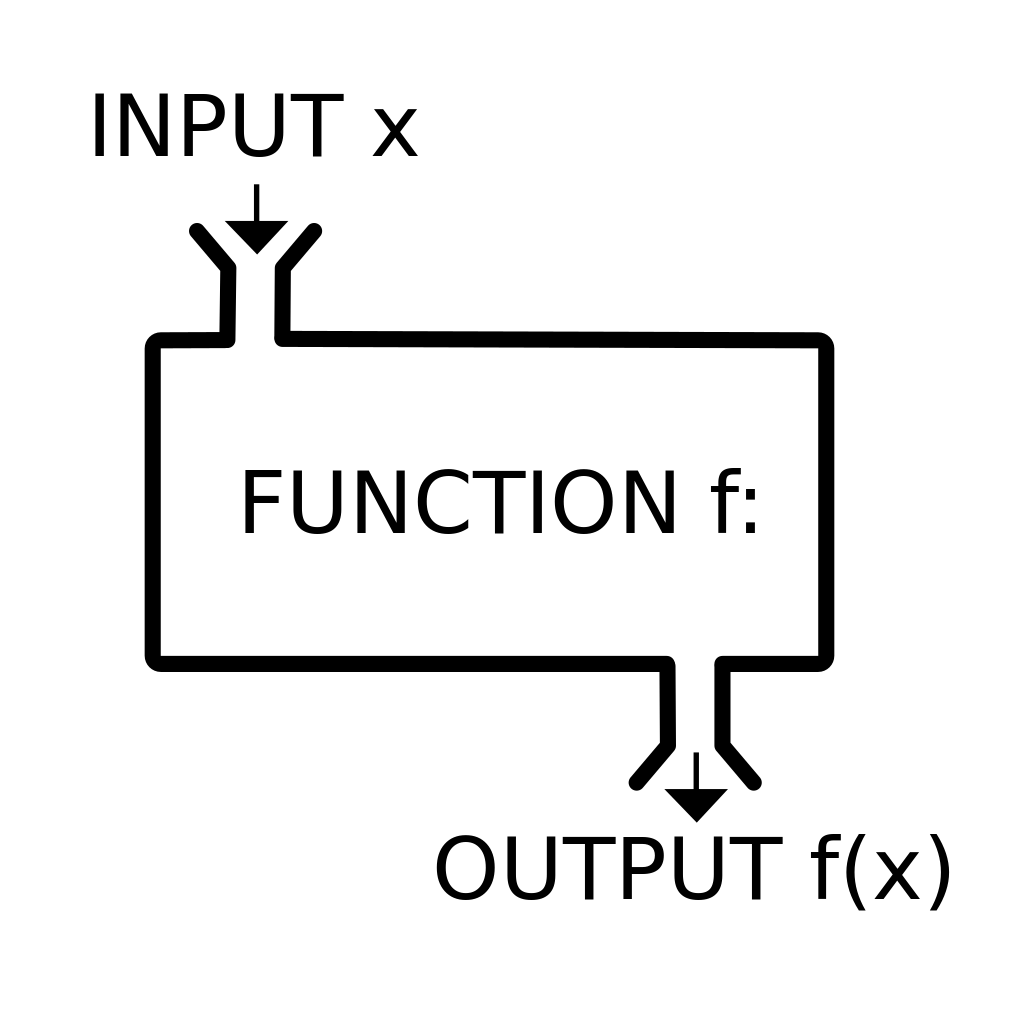
\includegraphics[width=0.5\linewidth]{math/19.png}
    \caption{Function as a black box}
    \label{fig:m19}
\end{figure}
\begin{equation}
    \text{For every } x \text{ there is one and only one } 
    F(x)
\end{equation}
In this case, we use $x$ as a variable, which means it assumes that we can plug anything into the function and it shapes into a "product". As the above definition stated, a function can only give one output for every input, so if you plug $1$ into $F(x)$, we will only get one output $F(1)$. 

\textbf{Domain} is the limit of what the functions can take ($x$). \textbf{Range} is the limit of what the function can give out as output (defined over $F(x)$). Both of them usually being defined with inequalities.

\textbf{Defining a function} is similar to defining a "procedure" to work on the input. In relationship terms, it is how the input is greater (addition), smaller (subtraction), many times bigger (multiplication), etc... Once again putting $x$ as the input, we can define $F(x)$ as an operation on our input:
\[ F(x) = 2x+1 \]
$F(x)$ \textit{depends} on the value of $x$ and the equation describes how those two relate.

\chapter{[Science] Significant Figures, Rounding, and Scientific Notation}
\textbf{Significant figures (digits)}, usually denoted with "SF" in Canada, is considered to be the level of precision of a number. The amount of significant figures you have implies the accuracy of your number. The rules are very easy to follow:
\begin{itemize}
    \item All \textbf{leading} zeros are not significant
    \item If there is a decimal point, all \textbf{trailing} zeros are significant
    \item Digits between the first and the last \textbf{non-zero digit} are significant
    \item If a digit is significant but the rules above do not cover, you can underline it
\end{itemize}
Remember, the second point only counts trailing zeros, which are zeros after a non-zero digit, regardless of where the decimal point is.

We can add "\textbf{plus/minus}" ($\pm$) to further show our level of accuracy.

\textbf{Rounding} is simply reducing the number of significant figures. Here is an additional rule you might not know about rounding 5: you should round it to make the last digit \textit{even}. This ensures that the ups and downs will cancel out each other over a long chain of calculations.

\section{Scientific notation}
Scientific notation is a way to deal with very big or very small numbers. There are two parts in a scientific notation: the \textbf{mantissa} $m$ (decimal portion) and the \textbf{exponent} $n$ (ordinate):
\begin{equation} m \times 10^n \end{equation}
A good way to think of the exponent $n$ is in terms of how you move the decimal point in the mantissa $m$. If $n$ is positive, move the decimal point to the right $n$ times (which is $\times10^n$), and vice versa for a negative power.

A constraint for the mantissa to prevent people from writing the number too hard to read is it must be between 1 and less than 10 ($1 \leq m < 10$). If you have $0.6$, simply move the decimal to the right and \textit{subtract} the exponent by $1$, which gives you $6\times10^{-1}$. A bit of simplification there because the whole number can also be negative, making the mantissa can be also negative ($-1.3\times10^1$ for example). When dealing with \textbf{negative scientific notation}, just treat it like a normal notation and do not confuse between negative mantissa and negative exponent.

\textbf{Ten raised by zero} equals 1, useful to represent numbers with the right mantissa but does not hint at the fact that it is in scientific notation:
\begin{equation} 10^0=1 \end{equation}

\textbf{To convert a number to scientific notation}, simply move the decimal point until it satisfies the mantissa's requirement. To remember which sign to put for the exponent: if you moved the decimal point to the left (making the mantissa smaller), then you need to multiply it by a factor of $10$ to make it the same as the original number. Ask yourself: do I need the exponent to be \textit{bigger} or \textit{smaller} to make the mantissa equal the original number?

Scientific notation is helpful when counting significant figures because now all of the digits that appear in the mantissa are significant.

\textbf{To add/subtract} numbers in scientific notation, make the exponent the same and simply deal with the mantissa, then readjust the result to proper scientific notation by moving the decimal. The answer should be rounded to the least number of decimal places.
\[\begin{aligned}
    & 3.0 \times 10^2 + 6.4 \times 10^3 \qquad 300 + 6400 \\
    =& 3.0 \times 10^2 + 64 \times 10^2 \qquad \text{least number of decimal places is }0 \\
    =& (3.0 + 64) \times 10^2 \\
    =& 67.0 \times 10^2 \qquad \text{round the number, return the mantissa to scientific notation} \\
    =& 6.7 \times 10^3
\end{aligned}\]

\textbf{To multiply/divide}, you also multiply/divide the mantissa by themselves first, then multiply/divide the exponents by using an exponent rule $10^n\cdot10^m=10^{n+m}$. This was hidden behind the fact that multiplication is commutative. The answer should have the same significant figures as the number with the least significant figures.
\[\begin{aligned}
    & (4.1\times10^6)\times(3.110\times10^8) \qquad\text{2SF} \times\text{4SF} \\
    =& (4.1\times3.110)\times10^{6+8} \\
    =& 12.751\times10^{14} \qquad \text{round to 2SF and shift decimal point} \\
    =& 1.2\times10^{15}
\end{aligned}\]

\chapter{Complex Numbers}
\section{Introduction}
The definition of a \textbf{complex number}:
\begin{equation} i = \sqrt{-1} \end{equation}
\begin{equation}
    \label{eq:m1}
    z = a + ib \in \mathbb{C}
    \qquad (a, b \in \mathbb{R})
\end{equation}
We define the real part of $z$ as $Re(z)=a$ and the imagined part $Im(z)=b$. Furthermore, we define the conjugate of a complex number as $z^*$ (z star):
\begin{equation} z^*=a-ib \end{equation}
Because $b=0$ for real numbers, the conjugate of a real number is itself.

\section{Visual intuition}
\begin{figure}
    \centering
    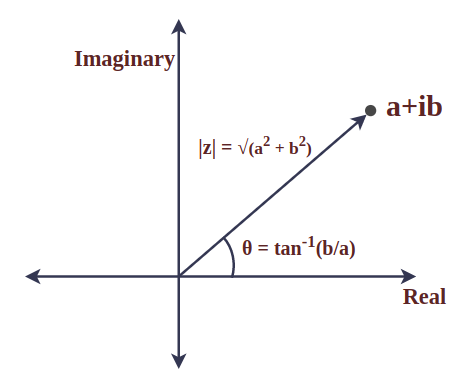
\includegraphics[width=0.5\linewidth]{math/9.png}
    \caption{Complex number intuition}
    \label{fig:m9}
\end{figure}
As a way to draw it on a standard two-axis graph similar to figure \ref{fig:m9}, you can put the horizontal axis (x-axis) as $a$ and the vertical axis as $b$ to represent the imaginary part of a complex number. This works better if you also recall that we were taught real numbers on a left-right number line. 

With this intuition, a number will have a certain "distance" away from the origin. When finding the conjugate of a complex number, you are essentially flipping the vertical axis. If you pay close attention to equation (\ref{eq:m1}), you can see that it closely resembles the standard graph form $y=mx+b$.

\section{Identities}
The \textbf{norm} of a complex number, which visually is the length of the vector from the origin to $z$ on a plane, is denoted as $\mid z \mid$:
\begin{equation} 
    \mid z \mid
    = \sqrt{a^2 + b^2}
\end{equation}
Another fundamental equation is \textbf{the norm squared} which is the direct result of the norm itself:
\begin{equation}
    \mid z \mid^2
    = a^2 + b^2
    = (a + bi)(a - bi)
    = z \cdot z^*
\end{equation}
The proof for these identities can be worked backward. Furthermore, the norm squared is used to calculate the probability of a state in quantum physics, something you should keep at the back of your mind if you want to pursue that field. 

From the visual intuition we established above, a complex number represented on a unit circle (the norm is equal to 1) can also be written with trigonometric functions:
\begin{equation}
    z
    = \cos{\theta} + i \sin{\theta}
    = e^{i\theta}
\end{equation}

\section{Complex number calculations}
\textbf{Adding and subtracting} two complex numbers is just simply doing every part individually:
\begin{equation} (a + bi) + (c + di) = (a + c) + (b + d)i \end{equation}
Remember to pay close attention to the negative sign at the beginning of the second term when subtracting.

\textbf{Multiplying} two complex numbers is simply using FOIL (multiplying terms together). Another extended version of FOIL that requires a bit of memorization is:
\begin{equation}
    (a+bi)(c+di)
    = ac + adi + bci + bdi^2 
    = (ac - bd) + (ad + bc)i
\end{equation}
A fascinating fact is when you multiply a complex number by $i$, the result is another complex number vector that is $90^\circ$ (or $\pi/2$) counterclockwise.

\textbf{Dividing} is a bit of work. You start with a fraction, then multiply the first fraction by another fraction with both the numerator and the denominator as the conjugate of the first fraction's denominator (making the second fraction equal to 1). Here is an example:
\[\begin{aligned}
    &\frac{2 + 3i}{4 - 5i} \\
    =& \frac{2+3i}{4-5i} \cdot \frac{4+5i}{4+5i} \\
    =& \frac{(2 + 3i)(4 + 5i)}{4^2 + 5^2} \qquad (a + bi)(a - bi) = a^2 + b^2 \\
    =& \frac{8 + 10i + 12i - 15}{41} \\
    =& \frac{-7 + 22i}{41}
    = -\frac{7}{41} + \frac{22}{41}i
\end{aligned}\]

\section{Polar form}
The polar form provides you with another "description" of the very same point on the plane. Instead of identifying a point on the plane using the axes, we use the distance from the origin and the angle from the positive x-axis instead. Notation-wise, $r$ is the radius from the origin (the distance) and $\theta$ is the angle from the positive x-axis. We can do a conversion from \textbf{Cartesian to Polar}:
\begin{equation}
    r = \sqrt{x^2 + y^2}
    \qquad
    \theta = \tan^{-1} (y/x)
\end{equation}
From \textbf{Polar to Cartesian}, we can calculate the $x$ and $y$ separately using $\cos$ and $sin$:
\begin{equation}
    x = r \times \cos\theta
    \qquad
    y = r \times \sin\theta
\end{equation}

A common way to write a complex number in Polar form from equation (6) is by getting the unit vector multiplied by the radius:
\begin{equation} x + iy = r(\cos\theta + i\sin\theta) \end{equation}

\section{Multiplying in Polar form}
The polar form provides intuition to complex multiplication problems. When multiplying two complex numbers together, the magnitudes get multiplied and the angles get added.
\begin{equation}
    \label{eq:m2}
    r = r_1 \times r_2
    \qquad
    \theta = \theta_1 + \theta_2
\end{equation}

This also explains why multiplying with $i$ with get a complex number that is perpendicular to the start vector. $i$ simply added $90^\circ$ to the angle and kept the radius the same.
\begin{equation} 0 + 1i \Rightarrow r = 1 \qquad \theta = 90^\circ \end{equation}

From equation (\ref{eq:m2}), we can yield the general formula when raising  a complex number by an exponent, called \textbf{De Moivre's formula}:
\begin{equation}
    (r(\cos\theta + i\sin\theta))^n
    = r^n(\cos{n\theta} + i\sin{n\theta})    
\end{equation}
\[ \Rightarrow r_{result} = r^n \qquad \theta_{result} = n \times \theta \]

\chapter{Permutation and Combination}
The difference between \textbf{permutation} and \textbf{combination} is in the order. \textbf{Permutation is an ordered combination} or in other words, a combination does not concern the order.

\textbf{Order does not matter} here means that a 123 string is the same as a 213 string.

When approaching statistical problems relating to permutation or combination, the basic approach should be calculating every individual part that you can count, then dividing to remove the over-count or multiplying to compensate for the under-count. 

\section{Permutation}
\subsection{Permutations with repetition}
When $n$ is the number of elements and $r$ is how many times we can select the elements, the number of possible permutations we can have is:
\begin{equation} n^r \end{equation}

For example, every time we roll a dice, there are 6 possible results (faces). If we roll it once again, now there are 6 results for every previous roll's result $6\times6$. If we ask how many permutations there are after 3 rolls of dice, the result is $6^3=216$ permutations. Every time we roll the dice, there is the possibility that a face will repeat (hence repetition is allowed).

\subsection{Permutations without repetition}
Four people were tasked to line up in a straight line, how many possible line arrangements can we get? There are four possible people to stand at the first position; for every selection, there will now be three possible candidates to stand at the second position, and so on... A person cannot appear twice in a line (not a quantum physics topic) so our choice gets reduced each time.

The formula is:
\begin{equation}
    n!
    = n \times (n-1) \times \dots \times 2 \times 1
\end{equation}
and despite being unrelated to statistics, this is a property of factorial:
\begin{equation} 0! = 1 \end{equation}

Continuing with the example above, what if we want to find how many possible line arrangements with only two people? In this question, we are "cutting short" our factorial formula because there are no more selections after the second person. To do that, we cancel the spare part by dividing it by itself:
\begin{equation}
    P(n,r) = nPr = P^r_n 
    = \frac{n!}{(n-r)!} = n(n-1)\dots(n-r+1)
\end{equation}
$n \ge r$ as you cannot have a collection longer than the number of elements you have. In this formula, the second notation was commonly seen on calculators, while the third notation is common in Vietnam (with $P$ being replaced with $A$).

\section{Combination}
The most common version you will need is combinations without repetition, so treat the combination with repetition as some extra reading.

\subsection{Combinations without repetition (regular combination)}
We want to pick two people from four people. We do not care about the order we pick but rather how many people we pick. Say if we picked Luke and Luna:
\begin{itemize}
    \item \textit{If the order does matter}: there are two possibilities: Luke first or Luna first.
    \item \textit{If the order does not matter}: only one possibility: Luke and Luna.
\end{itemize}
So as you can see, permutations have twice the possibilities. You can calculate how many possibilities permutation has \textit{more} than combination by using permutation on the subset itself (in this case, the set contains Luke and Luna):
\[ P(r, r) = r! \]
Now we simply divide our permutation formula with this spare part to get our \textbf{combination formula}:
\begin{equation}
    C(n,r)= nCr = C^r_n
    = \begin{pmatrix} n \\ r \end{pmatrix}
    = \frac{n!}{r!(n-r)!}
\end{equation}

You still need to keep in mind the fact that if an item was selected, it cannot be selected again in this non-repetition version (our example selection cannot have two Lukes or Luke will have to do a job twice).

\subsection{Combination with repetition}
This is a combination without repetition, but we plug in a different number to achieve our goal. Unfortunately, it is quite difficult to explain the algebraic proof so instead, this section will based on the visual intuition of one particular example.

We want to buy six tea bags, with three different flavours: (A) aloe vera tea, (B) black tea, or (C) chai tea. In this case, there are two important factors:
\begin{itemize}
    \item Repetition is allowed: we can pick a tea flavour more than once
    \item The order does not matter: we only care about how many we have picked
\end{itemize}

Because order does not matter, we will list our teas in the same order: A then B then C. Next, we will add a separator between the teas. Here is what our diagram will look like:
\[\begin{bmatrix}
    -&-&-&|&-&-&|&- \\
    |&-&-&-&|&-&-&- \\
    |&-&-&-&-&-&-&| \\
    |&|&-&-&-&-&-&-
\end{bmatrix}\]
There are still six dashes representing our six allowed selections, while the two separators simply indicate that we are moving between the types of tea. In the second example, you can see that we did not select A but only B and C. The third example only shows that there was only B that was selected; similar to C in the fourth example

With that diagram, the answer broke down to how many ways we can put down these two dividers. We have $n=3$ teas which means we have $n-1$ separators; There are $r+n-1$ spaces including the items and the separators to insert the divisors:
\begin{equation}
    C(n+r-1,n-1)
    = \frac{(n+r-1)!}{r!(n-1)!}
\end{equation}
This calls: select space to insert $n-1$ separators. Now you may ask why it is not simply $r-1$ (the space between the items only). It is because we always have the possibility that two separators are standing next to each other — such a case would 
 not be covered by the $r-1$ where there is no "space" for the separators to stand next to each other. 

The $n-1$ on the denominator gets from $n+r-1-r$ being cancelled, therefore we have the official \textbf{combination with repetition} formula:
\begin{equation}
    C(n+r-1,r) = C(n+r-1,n-1)
\end{equation}

The first hint to realize that you are dealing with combinations without repetition is in the fact that $n<r$. In our example, we had more positions to fill than the items we had, so we must repeat some. Notice that in this case, $n$ and $r$ "swapped" places for each other compared to other formulas; what we plugged in our original combination formula is still the same though.

\section{Solving problems}
\textbf{How many ways we can rearrange the word "Canada"?} This question cares about the order, so the first step is to get the basic permutation with the factorial formula $6!=720$. However, notice that there are three different "a" inside that word, so we need to "remove" that over-count. We do that by dividing our over-count by the number of possible arrangements of the three "a" characters:
\[ \frac{6!}{3!} = 240 \]

Most of the time when solving statistical problems, it is about you determining how much you have over-counted, then removing that spare part by dividing. 

\textbf{From 1,2, 3, and 4, how many 3-digit numbers (with non-repeating digits) can we get that are smaller than 320?} The first digit of our number will need to be either 1 or 2 to be \textit{certain} that any number selected after it will be smaller than $320$. Because this is non-repeating, after we select either 1 or 2, we only have $3$ options left for the second digit, and $2$ options for the last digit; the number of possibilities is: $2\times3\times2$. \textit{If the first digit is 3}, there is only one possibility for the second digit: 1 because otherwise, the number would be larger than $320$. The final result for this route can be calculated with $1\times1\times2$ or can be counted by listing $312$ and $314$.
\[ (2\times3\times2) + (1\times1\times2) = 14 \]

For this problem, an addition was used because we counted by part instead of under-counting every possibility. One thing to highlight this type of problem is when your logic route has conditional statements "if".

In both questions, we solved not by blindly applying the permutation or combination formula but rather by starting from scratch. This is extremely useful to help you keep track of what you are counting or for problems with multiple datasets to consider. 

\chapter{Limit}
Despite the author trying their best to explain this chapter for complete beginners, it is still expected that the reader has some basic understanding of limits. Please go read about limits somewhere first before hopping on this guide.

\section{Approach and limit}
\textbf{Approach} is the concept that a variable reaches closer and closer to a number. \textbf{Limit} is both the upper bound and the lower bound of something, like my patience for example. If we consider $x$ as the input and the value of $f(x)$ as the output, then we think limit as the bound for which the output could be given an input. 

Say we have a function that spreads one butter cube into two slices of bread ($g(x)=2x$). As we get closer and closer to two cubes ($x\to2$), then the number of bread slices we can spread will approach four slices. Represent that in a mathematical term, we have:
\[ \lim_{x\to2}g(x) = 4 \]

You may wonder: why I said that the limit is \textit{both} the upper and the lower bound but my result only gives out one value. This is because the difference between the upper bound and the lower bound is \textit{approaching} one single number. If you have two butter cubes, both the maximum and the minimum you can spread is 4. Later you will see that is not always true for certain equations.

Another interesting thing is that the limit is essentially what the value of the function \textit{is supposed} to be. In our case, we evaluate that limit by simply plugging $g(2)=4$. This is the property we got from the definition of limit itself: it is the "restriction" of the y-axis (the output) as the x-axis (the input) gets closer to a value (figure \ref{fig:m2}). If x "squeeze" then it will result in $g(x)$ being squeezed to a value. This is why when solving limits, it is about arranging your function to the point where you can plug in the $x$ value to answer your limit.
\begin{figure}
    \centering
    \begin{minipage}{.4\textwidth}
        \centering
        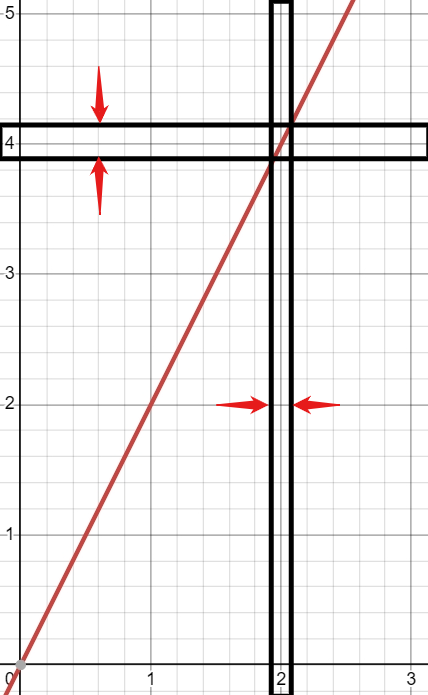
\includegraphics[width=0.9\linewidth]{math/2.png}
        \caption{Representation of $\lim_{x\to2}g(x)=4$}
        \label{fig:m2}
    \end{minipage}
    \begin{minipage}{.4\textwidth}
        \centering
        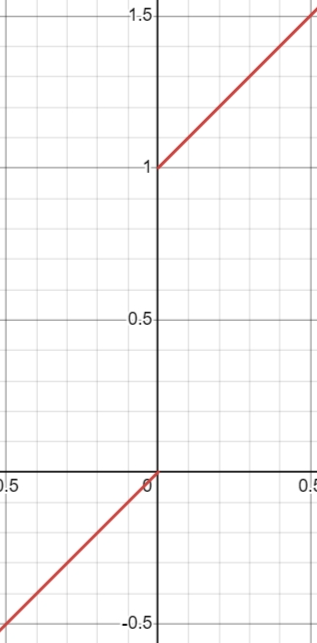
\includegraphics[width=0.75\linewidth]{math/3.png}
        \caption{A discontinuous function}
        \label{fig:m3}
    \end{minipage}
\end{figure}

The biggest takeaway from this section is: limit is what the output approaches given the input is approaching a number. Moreover, because both the upper bound and the lower bound approach a number, we can think of the limit as a value that the function is supposed to be at a given x-coordinate, even if the function is undefined at that point.

\section{Limit from different sides}
The example above "squeezes" the x-axis from both sides but what if we have an equation like figure \ref{fig:m3}?

No matter how hard you push the x-axis from two sides together, the y-axis limit will not get smaller. If we let $x$ approach from the left side (\textbf{negative side}) then the limit approaches $0$; if we let $x$ approach from the \textbf{positive side} then the limit approaches $1$. This is the situation we mentioned earlier about the upper bound and the lower bound creating a range instead of approaching one single number. In this case, we can only state what the limit approach as $x$ approaches from either side:
\[
    \lim_{x\to0^-}f(x) = 0
    \qquad
    \lim_{x\to0^+}f(x) = 1
\]
Be careful: the sign denotes where we \textit{start}. If the sign is negative, we approach it \textit{from the negative side} and move \textit{to the positive side}. I do not know why I used to mistake between those two, so that is a way to remember. Moreover, the limit of $f(x)$ as $x\to0$ does not exist.

A function's limit only exists if the limit from both sides approaches the same number:
\[
    \text{If }
    \lim_{x\to a^-}f(x)
    = \lim_{x\to a^+}f(x)
    \text {  then }
    \lim_{x\to a}f(x) \text{ exists}
\]
This leads us to the definition of \textbf{continuity}: if the limit of $f(x)$ at $a$ is equal to $f(x)$ then the function is continuous at $a$.

\section{Unbound limit}
\begin{figure}
    \centering
    \begin{minipage}{.5\textwidth}
        \centering
        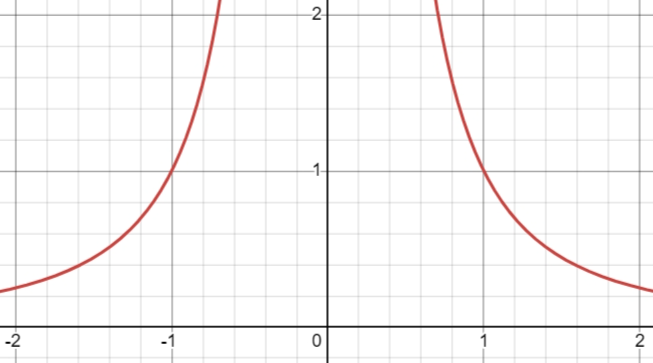
\includegraphics[width=0.9\linewidth]{math/1.png}
        \caption{The graph of the function $f(x)=\frac{1}{x^2}$}
        \label{fig:m1}
    \end{minipage}%
    \begin{minipage}{.5\textwidth}
        \centering
        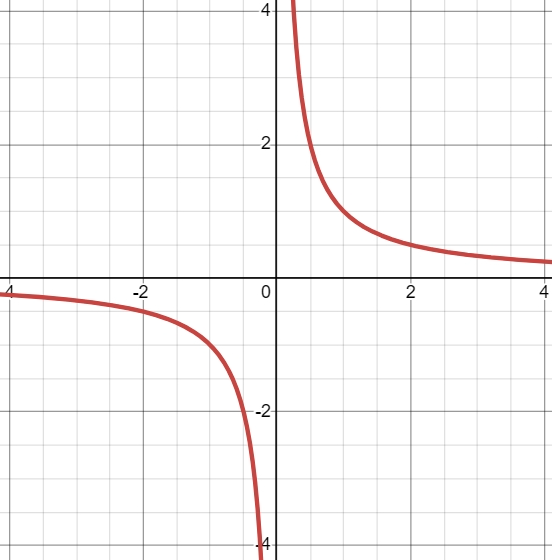
\includegraphics[width=0.9\linewidth]{math/4.png}
        \caption{The graph of function $f(x)=\frac{1}{x}$}
        \label{fig:m4}
    \end{minipage}
\end{figure}

Consider the function $f(x)=1/x^2$ in figure \ref{fig:m1},  you can see that moving from both sides, the limit slowly becomes higher and higher. It seems like it is \textbf{unbounded} or the limit seems to reach \textbf{positive infinity}.
\[ \lim_{x\to0} \frac{1}{x^2} = \infty \]

As you can see, both the upper limit and the lower limit still attempt to reach closer to one single value, so the limit still exists. Consider $f(x)=1/x$ in figure \ref{fig:m4}, we have the following:
\[
    \lim_{x\to0}\frac{1}{x} \textbf{ does not exist, but}
\]
\[
    \lim_{x\to0^-}\frac{1}{x} = -\infty
    \qquad
    \lim_{x\to0^+}\frac{1}{x} = +\infty
\]
The main limit does not exist, but the limit from either side is unbounded. The limit must exist first before continuing to check if the limit is bounded or unbounded.

\section{Limit to infinity}
Once again consider the function $f(x)=1/x^2$ as $x\to\infty$. What that means is we consider $x$ to grow to a big number and see if our y-axis merges to a number. From the graph, we can see that the value of the function is slowly reaching $0$, therefore we can state:
\[ \lim_{x\to\infty} \frac{1}{x^2} = 0\]

Of course, the limit to infinity can be infinity too:
\[ \lim_{x\to\infty} 2x = \infty \]

Do not be fooled! Infinity is not a variable you can move around or do mathematical operations to it. The equal sign in this case simply states that the limit is reaching a \textit{concept} of extremely big numbers. We will discuss more about evaluating limit to infinity in the evaluating section. You just need to remember that the limit to infinity simply assumes that as we plug large numbers, we look if the value of the function reaches a number or not.

\section{Solving finite limits}
If we have $c$ is a constant, $a$ is the number we are trying to approach, and we definite:
\[
    \lim_{x\to a}f(x) = L
    \text{ and }
    \lim_{x\to a}g(x) = M
\]
The basic \textbf{limit theorems} are:
\begin{equation}
    \lim_{x\to a}[f(x)+g(x)] = L+M
    \qquad
    \lim_{x\to a}[f(x)-g(x)] = L-M
\end{equation}
\begin{equation}
    \lim_{x\to a}[f(x)\cdot g(x)] = L\cdot M
    \qquad
    \lim_{x\to a}[f(x)/g(x)] = L/M
\end{equation}
\begin{equation}
    \lim_{x\to a}c = c
\end{equation}
\begin{equation}
    \lim_{x\to a} \left[f(x)^n\right]
    = \left[\lim_{x\to a}f(x)\right]^n
    \qquad
    (n \in N)
\end{equation}
These theorems can be deducted from the concept that limit is essentially substituting $a$ into our functions, so all standard number arithmetic still works just fine.

From these theorems, you can see that \textbf{finding a finite limit} is simply doing algebra manipulation of the function until you reach a point where you can substitute $x$ into your equation. The typical procedure to solve a finite limit can be found in figure \ref{fig:m5}. 
\begin{figure}
    \centering
    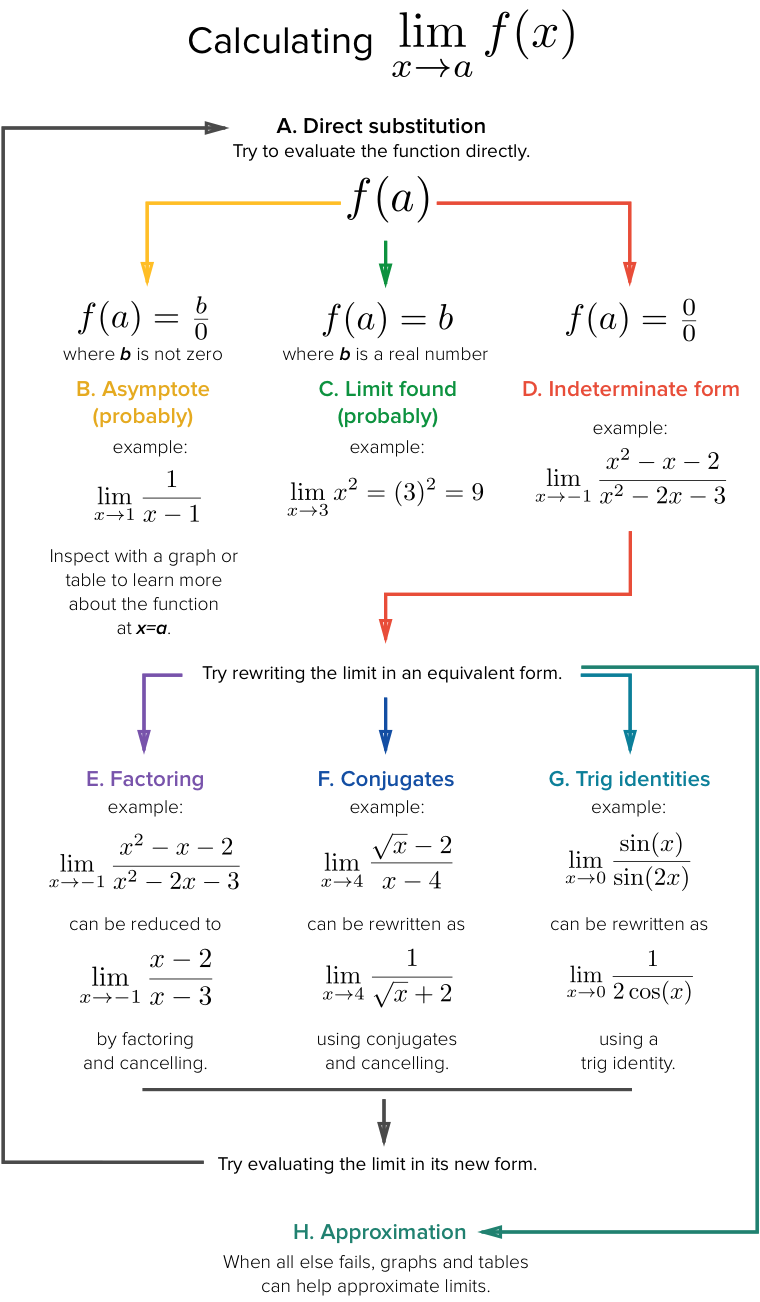
\includegraphics[width=0.75\linewidth]{math/5.png}
    \caption{Procedure to calculate limit, courtesy of Khan Academy.}
    \label{fig:m5}
\end{figure}

\subsection{Vertical asymptote}
The tables in this section use $+$ simply to denote the fact that the number is $>0$ and similarly with the negative sign.

\textbf{The limit of the multiplication between two functions}, when it is at the asymptote, can be simplified in table \ref{tab:m1}. Remember that multiplication is commutative and check if the limit exists in the first place or not. The table is pretty straightforward, as the signs are similar to multiplication between two numbers: two negatives get a positive.
\begin{table}
    \centering
    \begin{tabular}{|c|c|c|} \hline 
         $\lim_{x\to a}f(x)$ &$\lim_{x\to a}g(x)$ & $\lim_{x\to a}[f(x)\cdot g(x)]$\\ \hline 
         $+\infty$ & $+$ & $+\infty$\\ \hline 
         $+\infty$ & $-$ & $-\infty$\\ \hline 
         $-\infty$ & $+$ & $-\infty$\\ \hline 
         $-\infty$ & $-$ & $+\infty$\\ \hline
    \end{tabular}
    \caption{Finding the limit of the multiplication between two functions}
    \label{tab:m1}
\end{table}

\textbf{The limit of a division between two functions} $f(x)$ and $g(x)$ starts with two requirements:
\[
    \lim_{x\to a}f(x) \neq 0
    \text{ and }
    \lim_{x\to a}g(x) = 0
\]
After that, you need to check if the function $g(x)$ for $x$ approaches $a$ is larger than $0$ or not — you are checking the result that the whole function will dispense. The interaction between the limit of $f(x)$ and the sign of $g(x)$ can be found in table \ref{tab:m2}. Note that you still need to pay close attention to which direction you are approaching $x$ and whether the limit exists at that point. Once again the signs are similar to typical division.
\begin{table}
    \centering
    \begin{tabular}{|c|c|c|} \hline 
        $\lim_{x\to a}f(x)$ & The sign of $g(x)$ & $\lim_{x\to a}\frac{f(x)}{g(x)}$ \\ \hline 
        $+$ & $+$ & $+\infty$ \\ \hline 
        $+$ & $-$ & $-\infty$ \\ \hline 
        $-$ & $+$ & $-\infty$ \\ \hline 
        $-$ & $-$ & $+\infty$ \\ \hline
    \end{tabular}
    \caption{Interaction of the limit between two functions}
    \label{tab:m2}
\end{table}

\subsection{Trigonometric identities}
As it is impossible to cover all of the identities, this section will list identities that are useful in AP Calculus exams. First, recall the definition of a few trigonometric functions:
\begin{equation}
    \tan\theta = \frac{\sin\theta}{\cos\theta}
    \qquad
    \cot = \frac{1}{\tan\theta} = \frac{\cos\theta}{\sin\theta}
    \qquad
    \csc\theta = \frac{1}{\sin\theta}
    \qquad
    \sec\theta = \frac{1}{\cos\theta}
\end{equation}

Here are \textbf{Pythagorean identities}, which help when reviewing with a unit circle that displays trigonometric functions like figure \ref{fig:m8}:
\begin{figure}
    \centering
    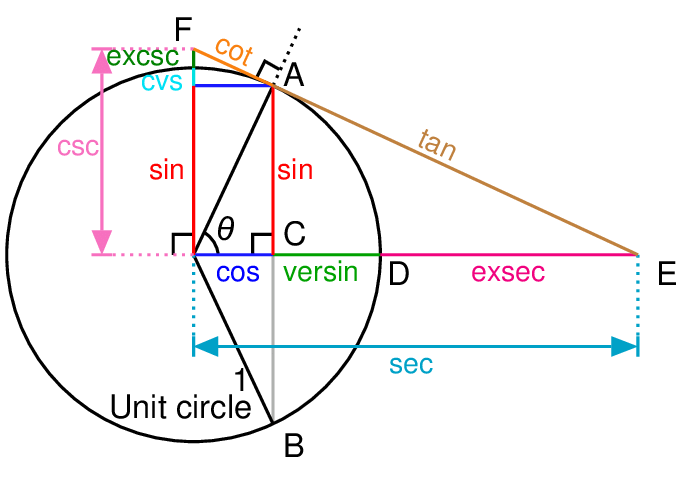
\includegraphics[width=0.75\linewidth]{math/8.png}
    \caption{A unit circle with trigonometric functions}
    \label{fig:m8}
\end{figure}
\begin{equation}
    \sin^2\theta + \cos^2\theta = 1^2
    \qquad
    \tan^2\theta + 1^2 = \sec^2\theta
    \qquad
    1^2 + \cot^2\theta = \csc^2\theta
\end{equation}
The $1^2=1$ was added to help the reader remember the connection to the original Pythagorean theorem $a^2+b^2=c^2$. You can work out more identities from the figure. Just in case you forgot, $\sin^2\theta=\sin(\theta)\cdot\sin(\theta)$ — it is the squared of the \textit{result} of the function, NOT the $\theta$ inside the function.

The \textbf{double-angle identities}:
\begin{equation}
    \sin2\theta = 2 \sin\theta \cos\theta
\end{equation}
\begin{equation}\begin{aligned}
    \cos2\theta
    =& \cos^2\theta - \sin^2\theta \\
    =& 2\cos^2\theta - 1 \\
    =& 1 - 2\sin^2\theta
\end{aligned}\end{equation}
\begin{equation}
    \tan2\theta = \frac{2\tan\theta}{1 - \tan^2\theta}
\end{equation}

The \textbf{half-angle identities} frequently being mentioned but more often used for integral questions:
\begin{equation}
    \sin^2\theta = \frac{1}{2}(1-\cos2\theta)
\end{equation}
\begin{equation}
    \cos^2\theta = \frac{1}{2}(1+\cos2\theta)
\end{equation}

Finally, it is crucial to remember that the limit of most of the trigonometric functions as $\theta\to0$ is undefined. Can you see why?

\subsection{Composite function limits}
The standard theorem is:
\begin{equation}
    \lim_{x\to a} f(g(x))
    = f(\lim_{x\to a} g(x))
\end{equation}
If and only if the limit of $g(x)$ exists and $f(x)$ is continuous at $\lim_{x\to a} g(x)$:
\[
    \lim_{x\to a}g(x) = L
    \text{ and }
    \lim_{x\to L} f(x) \text { exists}
\]

Remember: the theorem only stated about "moving" the limit inside and does not mention anything about the limit itself. Therefore, if you cannot apply the theorem, it does not mean that the limit does not exist so you should inspect the function instead. 

When inspecting the functions through graphs, it is best to put the two functions in two different graphs. Since the output of $g(x)$ is the input of $f(x)$, you can visualize it as if you "flip" the $g(x)$ y-axis to match with the x-axis of $f(x)$.

Finally, if the graph is discontinuous, it does not mean that the limit at that point does not exist. Slowly follow one-sided limits and see if they are equal.

\subsection{The squeeze theorem}
Also known as the \textbf{sandwich theorem}, it helps calculate limits that are a bit weird. Suppose in an area that we know:
\[ f(x) \leq h(x) \leq g(x) \]
then for some real number $a$:
\begin{equation}
    \text{If } \lim_{x\to a}f(x) = L = \lim_{x\to a}g(x)
    \text{ then }
    \lim_{x\to a}h(x) = L
\end{equation}
Read: If we certainly know that, inside the range we are evaluating, $h(x)$ is always between the other two functions, then if the limit of both $f(x)$ and $g(x)$ is equal to a number, then those two limits "sandwich" $h(x)$ to that same value.

For example, we have the following function with the graph from figure \ref{fig:m7} and \ref{fig:m6}:
\[ x^2 \sin\left( \frac{1}{x} \right) \]
\begin{figure}
    \centering
    \begin{minipage}{.4\textwidth}
        \centering
        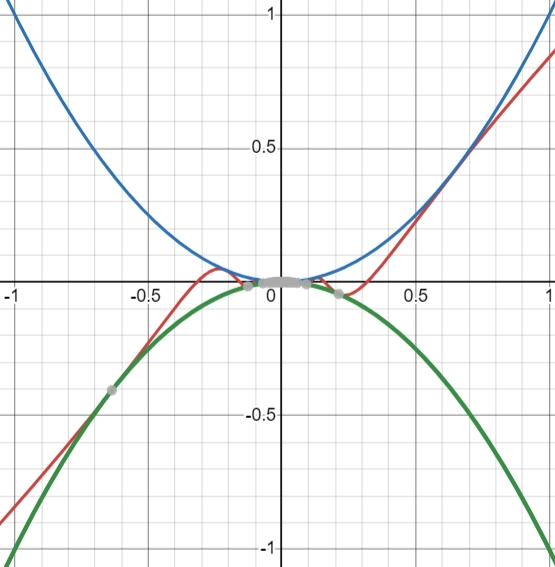
\includegraphics[width=0.75\linewidth]{math/7.png}
        \caption{The graph of $x^2\sin{\frac{1}{x}}$ and $\pm x^2$}
        \label{fig:m7}
    \end{minipage}
    \begin{minipage}{.4\textwidth}
        \centering
        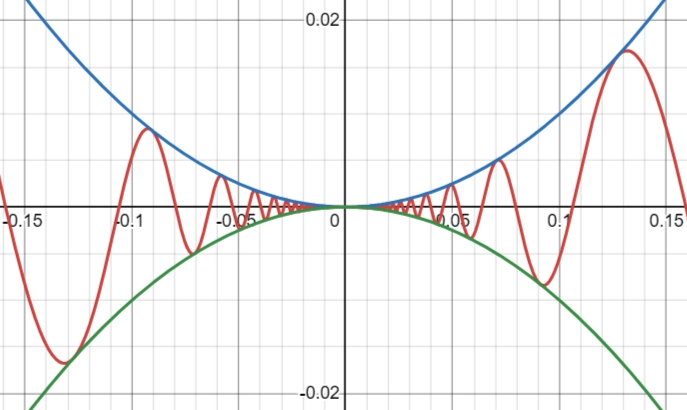
\includegraphics[width=1\linewidth]{math/6.png}
        \caption{The graph zoomed in}
        \label{fig:m6}
    \end{minipage}
\end{figure}

Of course, we can observe from the graph that the function approaches $0$ as $x\to0$, but what if we don't have the graph? We know from the property of a sine graph that the coefficient at the front will determine the height of the graph. Therefore, we know that:
\[
    -1 \leq \sin(x) \leq 1
    \Rightarrow
    -x^2 \leq x^2 \sin\left( \frac{1}{x} \right) \leq x^2
\]
And we know that at $0$, $-x^2 = x^2 = 0$, therefore making:
\[ \lim_{x\to0} x^2 \sin\left( \frac{1}{x} \right) = 0\]

\section{Solving limits at infinity}
There are two seemingly different ways to solve for infinite limits but behind the curtain, they are the same. 

The \textbf{intuitive way} is to turn the function into a rational function (a function in the form $P(x)/Q(x)$). If the degree of the numerator is higher, then the limit is either positive infinity or negative infinity — you need to look at the sign of the $x$ with the highest degree since that $x$ will be the one that determines the direction of the equation. If the degree of the denominator is the largest, then the limit will head to $0$. If the degree of both are equal, divide the coefficients of the terms with the largest exponent:
\[
    lim_{x\to\infty}\frac{-5x^2+1}{3x^2-x}
    = \frac{-5}{3}
\]

Finally, you can combine with the theorems mentioned above to adjust your answer properly. The reason this works is we are trying to find which term grows the fastest by comparing their degree; if they have the same degree, they "contested" each other to reach a ratio.

The \textbf{algebraic way} is to transform what you have into what you can evaluate. All the theorems from the solving finite limit section still hold unless specified otherwise. 
\[\begin{aligned}
    & lim_{x\to\infty}\frac{5x^2+1}{3x^2-x} \\
    =& 
        lim_{x\to\infty}\frac{(5x^2+1) / x^2}{(3x^2-x) / x^2} 
        &\text{divide by } x^2 \\
    =& lim_{x\to\infty}\frac{5+\frac{1}{x^2}}{3-\frac{x}{x^2}} \\
    =& 
        \frac
            {lim_{x\to\infty}(5+\frac{1}{x^2})}
            {lim_{x\to\infty}(3-\frac{x}{x^2})}
        &\text{apply the theorems} \\
    =& \frac{5+0}{3-0} &\text{find the limit of each term} \\
    =& \frac{5}{3}
\end{aligned}\]

It is once again crucial to remember that you cannot simply substitute $\infty$ into your equation and manipulate it as if it is a variable.

\section{L'Hôpital's rule} \label{sec:m-limit-hopital}
If you think the derivative $f'(x)$ is simply a special transformation of the original function $f(x)$, we can use the derived function to solve a limit that is in the indeterminate form:
\begin{equation}
    \lim_{x\to a} \frac{f(x)}{g(x)}
    = \lim_{x\to a} \frac{f'(x)}{g'(x)}
\end{equation}
Here are the \textbf{indeterminate forms} that L'Hôpital rule can help with:
\begin{equation}
    \frac{0}{0} \qquad
    \frac{\infty}{\infty} \qquad
    0\times\infty \qquad
    1^\infty \qquad
    0^0 \qquad
    \infty^0 \qquad
    \infty - \infty
\end{equation}
The \textbf{conditions} are, very obvious, the functions must be differentiable and the final limit must exist. Less obvious is the fact that you can only use this rule when $f(x)/g(x)$ is indeterminate.

You can take as many differentiations as it takes to solve the limit equation. You can also take the antiderivative but usually, that will result in a more complex function. Consider we have this example:
\[
    \lim_{x\to\infty} \frac{e^x}{x^2}
    = \frac{\infty}{\infty}
\]
Note that the derivative of $e^x$ is $e^x$, we can slowly transform our limit:
\[
    \lim_{x\to\infty} \frac{e^x}{x^2}
    = \lim_{x\to\infty} \frac{e^x}{2x}
    = \lim_{x\to\infty} \frac{e^x}{2}
    = \infty
\]
In the last step, we know that $e^x$ grows much more rapidly than $2$.

\chapter{Derivatives}
It is recommended that the reader understand about limits before proceeding.

\section{Derivative concept}
Today is a beautiful day to find the slope of a graph at a point. We remember that the slope between two points is the difference in the y-axis divided by the difference in the x-axis:
\begin{equation}
    m
    = \frac{\Delta y}{\Delta x}
    = \frac{y_2-y_1}{x_2-x_1}
\end{equation}

However, what we originally asked is the slope of a graph at one single point, therefore we need to move the two points as close as possible to each other (\textit{the definition of limit}) until they are essentially one point similar to figure \ref{fig:m10}. Consider the fact that the y-axis essentially is the output of the function $f(x)$, making $\Delta y=f(x+\Delta x)-f(x)$, we can use limit to describe the fact that the difference $\Delta x$ is getting smaller and smaller ($\Delta x\to0$):
\begin{equation}
    \label{eq:m3}
    f'(x)
    = \lim_{\Delta x\to 0} \frac
        {f(x+\Delta x)-f(x)}
        {\Delta x}
\end{equation}
\begin{figure}
    \centering
    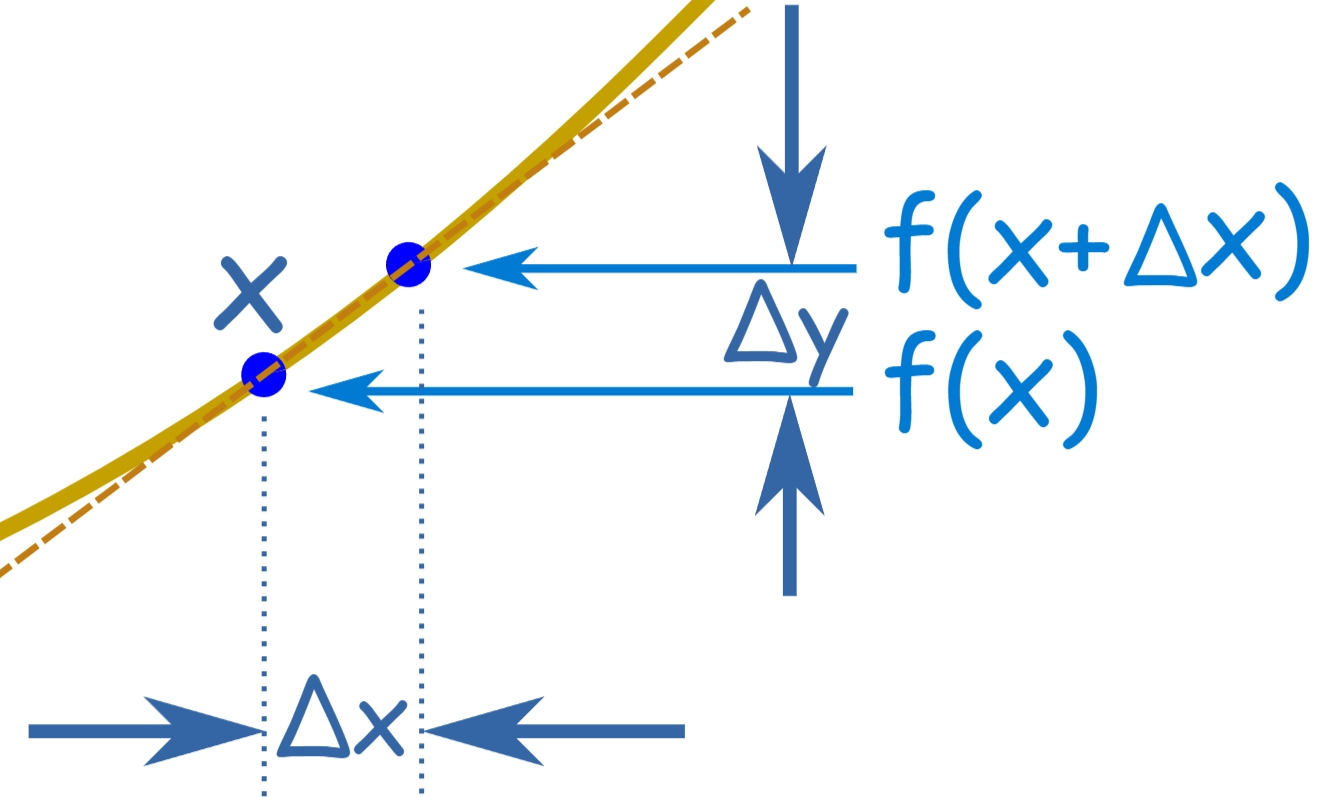
\includegraphics[width=0.5\linewidth]{math/10.png}
    \caption{Two points approaching each other, courtesy of Math is Fun}
    \label{fig:m10}
\end{figure}

Other notations to highlight the fact that the derivative is simply the rate of change of a function at a point is:
\begin{equation}
    \frac{d}{dx}f(x) = \frac{df}{dx} = \frac{dy}{dx}f(x)
\end{equation}
This notation highlights the fact that the derivative is the \textit{ratio} between the change in the y-axis and the change in the x-axis, giving you the ability to move $dx$ in the scenario of integrals, which you will learn later.

Lastly, you can take derivatives as many times as you like. After all, if you take the derivative of a derivative, it simply showing the rate of change of the derivative function itself.
\begin{equation}
    f''(x)=(f'(x))'
\end{equation}

\section{Derivative rules}
In this section, instead of using the full notation $f(x)$, the function is simplified to $f$. The start of this section will simply provide a quick look-up sheet of the rules, while the latter part will explain the intuition of some harder rules. 

A note: before you do any derivative manipulation, consider simplifying the function. For example, we have:
\[
    [(x+1)^2]' = [x^2 + 2x + 1]' = 2x + 2
\]
If you were to manipulate the original equation as a composite function the derivative would be much messier.

\textbf{Multiplication by a constant}:
\begin{equation} (cf)' = cf' \end{equation}

The \textbf{sum} and \textbf{difference rule} are a bit anti-climatic:
\begin{equation}
    (f+g)' = f'+g'
    \qquad
    (f-g)' = f'-g'
\end{equation}

The \textbf{product rule} can be remembered by the phrase "Left-D right, right-D left":
\begin{equation}
    (fg)' = fg'+f'g
\end{equation}

The \textbf{quotient rule} was found by expanding the derivative's limit definition. Unfortunately, this rule does not have any possible visualization so you might have to rote learn this:
\begin{equation}
    \left( \frac{f}{g} \right)'
    = \frac{f'g-fg'}{g^2}
\end{equation}

The \textbf{reciprocal rule} is another rule that is a bit hard to digest, but luckily rarely seen:
\begin{equation}
    \left( \frac{1}{f} \right)'
    = -\frac{f'}{f^2}
\end{equation}

It is also appropriate to recall the \textbf{fractional exponent rule} and \textbf{negative exponent rule}:
\begin{equation}
    a^\frac{m}{n} = \sqrt[n]{a^m}
    \qquad
    a^{-n} = \frac{1}{a^n}
\end{equation}
Which will be useful when utilizing \textbf{the power rule}:
\begin{equation} (x^n)' = nx^{n-1} \end{equation}
You can remember that the power rule "flattened" our exponent graph by one degree.

The \textbf{chain rule} in a wordy notation but the one that gets across my mind is: assume we have $u=g(x)$ and $y=f(u)=f(g(x))$ then the derivative is:
\begin{equation}
    y'_x
    = y'_u \cdot u'_x
\end{equation}
This means that "the derivative of $f$ plug in original $g$ times the derivative of $g$ plug in $x$". You can feel it showcases a "staircase" approach to the composite function.

The \textbf{L'Hôpital rule} is used when finding the limit at a point with an indeterminate result (read more about its usage in \ref{sec:m-limit-hopital} Limit chapter, L'Hôpital section):
\begin{equation}
    \lim_{x\to a} \frac{f(x)}{g(x)}
    = \lim_{x\to a} \frac{f'(x)}{g'(x)}
\end{equation}
This means the limit of a quotient of two functions equals the limit of the quotient of the derivative of those two functions.

When all rules fail, you can always use the original derivative definition in equation \ref{eq:m3}

\subsection{Visualizing the product rule}
% Maybe someday change f(x) to y and df to dy. I won't change it right now because that means redrawing figure m11.
Assume we have two functions: $g(x)$ and $h(x)$, and $f(x)=h\cdot g$. Because it is the multiplication between two functions, you can think of $f(x)$ as the area of a rectangle with $h(x)$ and $g(x)$ as two sides, similar to figure \ref{fig:m11}.
\begin{figure}
    \centering
    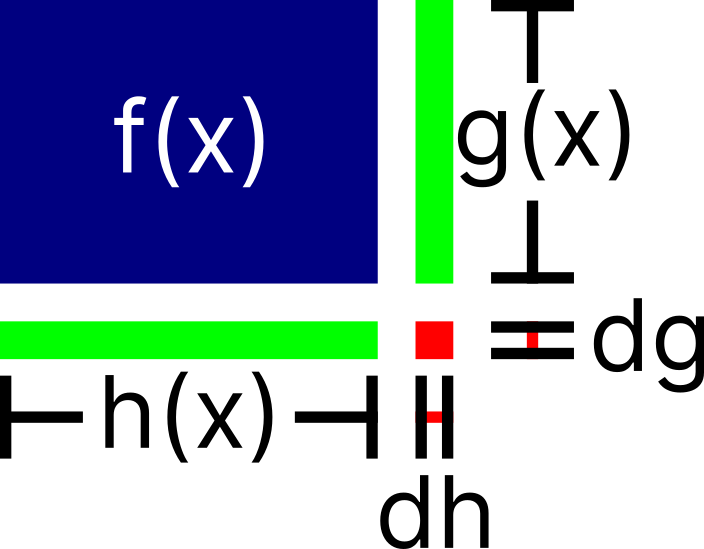
\includegraphics[width=0.5\linewidth]{math/11.png}
    \caption{Representation of a product between two functions}
    \label{fig:m11}
\end{figure}

To calculate the rate of change at that point, we need another point $dx$ away from $x$ and $dx\to0$. Furthermore, we need to consider how our two functions "react" to $dx$. We deduct from the formula of derivative:
\[
    \frac{dh}{dx} = h'
    \Leftrightarrow
    dh = h' \;dx
\]
A similar transformation can be made with $g(x)$. What $dh$ is showing here is how much the result of the function $h(x)$ would increase for a change in $x$ — $dh$ is the change we have when we move $x$.

Label the additional area $df$:
\[ df = g \cdot dh + h \cdot dg + dh \cdot dg \]
We can expand the entire equation to:
\[ df = g(h' \;dx) + h(g' \;dx) + (h' \;dx) \cdot (g' \;dx) \]
We want to find the ratio at that point $df/dx$, so we divide both sides by $dx$:
\[ \frac{df}{dx} = g \cdot h' + g' \cdot h + h' \cdot g' \;dx \]
Because $dx\to0$, we can eliminate that term:
\[
    \frac{df}{dx} = gh' + g'h
    \Rightarrow
    \frac{d}{dx}(gh) = gh' + g'h
\]

\subsection{Visualizing the chain rule}
An anonymous professor once said: "Using the chain rule is like peeling an onion: you have to deal with each layer at a time, and if it is too big you will start crying." 

Assume we have $g(h(x))$. We can imagine these two functions like a production line: we put in the raw number $x$, and then the function $h$ will "process" the input before passing it to $g$, after which the output will then be given. This production chain can be visualized in figure \ref{fig:m12}. Note that now we denote a tiny change in our input as $dx$, a tiny change in our output as $dy$, and our ultimate goal is to find the ratio $dy/dx$.
\begin{figure}
    \centering
    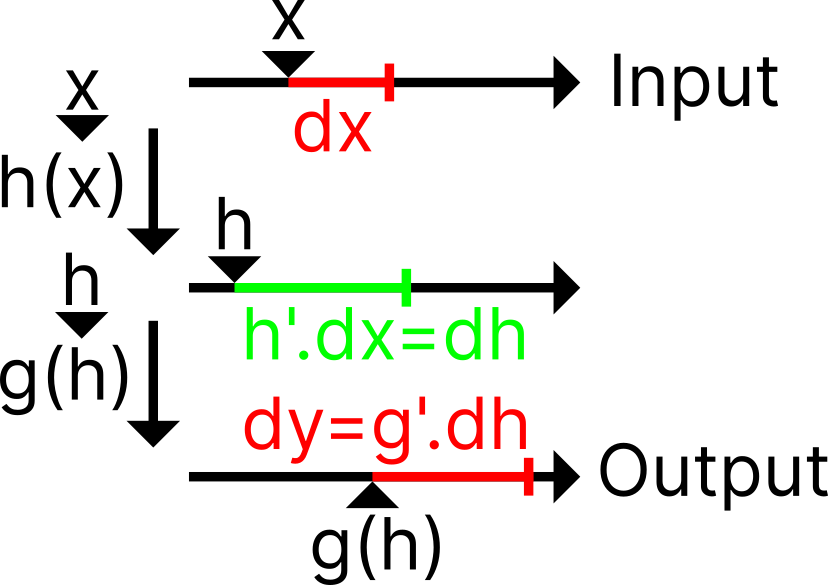
\includegraphics[width=0.5\linewidth]{math/12.png}
    \caption{Chain rule visualization}
    \label{fig:m12}
\end{figure}

As we increase our input by a $dx$ amount, it will increase the \textit{output} of the function $h$ by a $dh$ amount. Similar to the product rule, we manipulate our derivative ratio $dh/dx$ to calculate that change in the output:
\[ dh = h'(x) \;dx \]
Repeat that same process with the function $g$, but now you have to remember that the input is no longer $x$, but $h$ and a tiny change $dh$:
\[ dy = g'(h) \cdot dh \]
Expand $dh$, we have:
\[ dy = g'(h) \cdot (h' \;dx) \]
Finally, because we ultimately want to find the ratio of the changes, we divide both sides by $dx$ and expand the fact that $h$ is simply $h(x)$:
\[ \frac{dy}{dx} = g'(h(x)) \cdot h'(x) \]
If you think of  $dg/dh$ as "derivative of $g$ when plugging in $h$", another interesting way to write this:
\[ \frac{dy}{dx} = \frac{dg}{dh}\frac{dh}{dx} \]

\section{Derivative of common functions}
\textbf{A constant} will have a slope equal to $0$:
\begin{equation} (c)' = 0 \end{equation}

\textbf{A line} will have a slope similar to its... slope. This is similar to $m$ in the form $y=mx+b$:
\begin{equation}
    (ax)' = a
    \qquad
    (x)' = 1
\end{equation}

\textbf{The derivative of a square root:}
\begin{equation}
    \sqrt{x}
    = x^\frac{1}{2}
    = \frac{1}{2} x^{-\frac{1}{2}}
\end{equation}

\textbf{Exponential functions} with $x$ as the exponent. Further explanation can be found in Euler's constant and the natural $\log$:
\begin{equation}
    (e^x)' = e^x
    \qquad
    (a^x)' = a^x\ln(a)
\end{equation}

\textbf{Logarithms}:
\begin{equation}
    (\ln(x))' = \frac{1}{x}
    \qquad
    (\log_a(x) )' = \frac{1}{x\ln(a)}
\end{equation}

\textbf{Trigonometric functions}:
\begin{equation} 
    (\sin x)' = \cos x 
    \qquad
    (\cos x)' = -\sin x
    \qquad
    (\tan x)' = \sec^2x
\end{equation}

\section{Additional material}
It is recommended that you explore chapter \ref{sec:m-integral} for the \textit{inverse} concept of derivative: anti-derivative. For other additional reading material connecting to calculus as a whole, place look at the additional material section at \ref{sec:m-integral-material}.

\chapter{Integrals}\label{sec:m-integral}
It is an absolute requirement that the reader understands derivatives, which in turn requires the knowledge of limits. 

\section{Why antiderivative is integral?}
This section is not necessary to understand the concept of integral, so the reader feels free to skip it. However, this section will provide an in-depth examination of how mathematicians came up with the connection between antiderivative and integral — we are going to construct calculus from the ground up. If that is the question you have in mind, please continue to read this section as the author has rewritten it thrice now.

Assume we have a graph $f(x)$ and an unknown function $A(x)$ that represents the area under $f(x)$ between the y-axis and the input. We will split into two situations and each situation will explain a different component of integration to construct the full image:

\subsection{The main function is zero-degree (constant)}
If we have $f(x)=c$, the graph of our constructed function will look like figure \ref{fig:m13}. If we were to find the area between $0$ and $a$, we could simply calculate $A(a)$ to get the result.
\begin{figure}
    \centering
    \begin{minipage}{.4\textwidth}
        \centering
        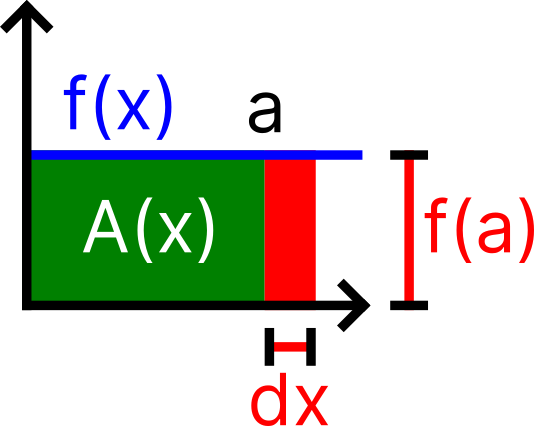
\includegraphics[width=0.9\linewidth]{math/13.png}
        \caption{A representation of a constant function's integral}
        \label{fig:m13}
    \end{minipage}
    \begin{minipage}{.4\textwidth}
        \centering
        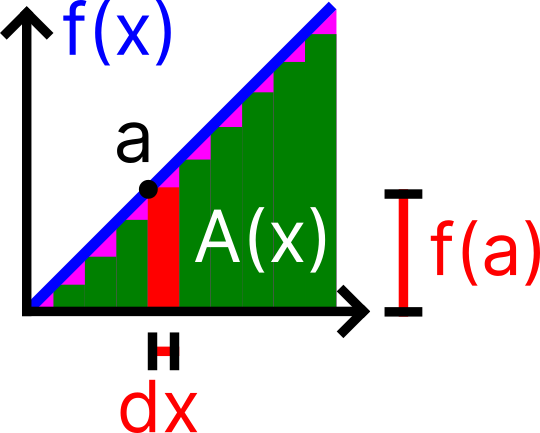
\includegraphics[width=0.9\linewidth]{math/14.png}
        \caption{A representation of a linear function's integral}
        \label{fig:m14}
    \end{minipage}
\end{figure}

If we move $a$ a $dx$ amount to the right and want to find the area at that point, we plug $A(a+dx)$. If you look at the red rectangle on the figure, there are two ways to interpret that area:
\begin{itemize}
    \item It is the area of $A(a+dx)$ subtracted by $A(a)$
    \item It is the area created by the increase in the variable $a$ (which is $dx$) multiplied by the height of that area $f(a)$ (in this case, we plug the number in to find the height).
\end{itemize}
And clearly, those two are mentioning the same area, so we can state that they are equal:
\[
    A(a+dx)-A(a)
    = f(a) \;dx
\]
We can generalize the point we selected by replacing $a$ with $x$:
\[
    A(x+dx)-A(x)
    = f(x) \;dx
\]
Then re-arrange the equation:
\[
    \frac{A(x+dx)-A(x)}{dx}
    = f(x)
\]
Hang on... that essentially stated that the slope of $A(x)$ is the value of $f(x)$; on the other hand, it stated that essentially $f(x)$ is the derivative of $A(x)$! Despite $A(x)$ being unknown in the beginning, we can find a function whose derivative is $f(x)$ to get $A(x)$. Thus, the antiderivative is the area under the graph.

\subsection{The main function is first-degree (linear)}
Alright, we have seen the connection between $A(x)$ and $f(x)$, but where are the $\int$ sign and the final $dx$? Assume $f(x)$ is a linear equation with a graph similar to figure \ref{fig:m14}. Notice that now our area function will need to account for both the green rectangle and the pink triangle at the top of every rectangle.

If we want to find the area under $f(x)$ from $0$ to $a$, we will need to add the area of all of the slices between $0$ and $a$. The area of each green rectangle is $f(x) \;dx$ and we want to find the sum of all of those areas from $0$ to $a$:
\[
    \int^a_0 f(x) \;dx + \text{pink area}
    = A(a)
\]
As you can see, the $\int$ acts both as a $\Sigma$ notation for the sum of the rectangles and $\lim_{dx\to0} f(x)\;dx$\footnote{This notation is semi-accurate for the sake of simplicity. If you want to understand integral as summation, search "Riemann sum".}. Intuitively, you can see that the slope of $f(x)$ will dictate how much the area will grow moving from $a$ to $dx$: the sharper $f(x)$ is, the faster the area will grow and reverse. The integral is the accumulation of change.

Note that the smaller the $dx$, the finer we slice our area, making our pink area approach $0$ and our summation of the green area closer to the actual area. Algebraically, this is because $f(x)=dA/dx$ so the left term will cancel out $dx$, while the pink area will still be multiplied by $dx$ (the base width of the triangle). Eventually, we have:
\[
    \int^a_0 f(x) \;dx
    = A(a)
\]

If we have another point $b>a$, and we want to find the area from point $a$ to $b$, we simply find the area of point $b$ and minus it by the area at $a$:
\[
    \int^b_a f(x) \;dx
    = A(b) - A(a)
\]

\section{Integration concept}
Starting with a geometry intuition: think of a paper. If you look at a paper from the edge, it has a very tiny thickness. However, as you stack the papers together, eventually those tiny thicknesses will create an area on the side: you can measure the height of the stack and multiply it by the edge's length to get the stack's edge area.

Integral is the \textbf{antiderivative} of a function, which helps us find the area under a curve by chopping it into thin sheets and stir-frying it... wait sorry wrong note... \textit{Ehem...}

Integral helps us find the area under a function $f(x)$ by slicing it into many small pieces with equal $dx$ thickness and height of $dx$. As $dx\to0$, our approximation of the area will get better and better; at some point with extremely small $dx$, the value would just be the sum of all small segments of $f(x)$. Similar to our paper example from above: as we continue to stack the papers, the sides will eventually create an area. To tell that $F(x)$ is the \textbf{indefinite integral} of $f(x)$, we use
\begin{equation}
    \int f(x) \;dx = F(x) + C
\end{equation}

The reason we have $C$ is because any constant will have its derivative as $0$, so both $F(x)+1$ or $F(x)+3$ will have the the derivative as $f(x)$. To express that we have a lot of possible antiderivatives, we use the constant $C$. \textit{When solving integrals}, most of the time you can simply add the integration constant at the very end when answering the question instead of accounting it for every small step.

The notation we used above is \textit{indefinite integral} which expresses a function without any particular input and does not spit out any number. If we want to find the area of a particular region $[a,b]$, we will use a \textbf{definite integral} to denote $a$ as the lower bound and $b$ as the upper bound. Since we have $F(x)$ as the area function from $0$ to $x$, we find the area of $[0,b]$ and then subtract it by $[0,a]$ to get the interested area:
\begin{equation}
    \int^b_a f(x) \;dx
    = \left. F(x) \right|^b_a
    = F(b) - F(a)
\end{equation}
Note that the $C$ was \textit{conveniently} cancelled, so we can ignore that.

Another important thing to remember is integral is the \textbf{signed area} under a function. What that meant is that if the function $f(x)$ ever dipped below $0$, then the area between the x-axis and $f(x)$ will be considered negative. If you want the area in general without that subtraction, consider splitting your integral into two: calculate the positive area then add it to the absolute value of the negative area.

\textbf{Notation-wise}, because integration is the sum of $f(x)\;dx$, it is also appropriate to remember that the $dx$ is still a part of the integral\footnote{Technically, you can still move the $dx$ outside of the integral since the $dx$ was distributed into multiple terms of $f(x)$, so you just need to symbolize the sum of all $f(x)$ then multiplied it to $dx$. However, this is a high-level technique and requires an in-depth understanding of this topic itself.}:
\[
    \int (f(x)\cdot dx)
\]
Please don't kidnap $dx$ in the dead of the night when you are doing homework that is due the next day. Only physicists do that\footnote{Feel free to contemplate on the equation $e^x=(1-\int)^{-1}0$ before contacting your local physicist.}. 

A final word of this section: \textbf{antiderivative (indefinite integral)} is simply the function $F(x)$ without any real value, while \textbf{definite integral} is the result of plugging in values into our indefinite integral. Those two terms are usually used interchangeably, but they are slightly different.

\section{Integration rules}
Note that the lowercase $c$ in this section is different from the integral constant $C$ (uppercase). Generally, the integral of a function will have a higher degree and will be a bit more complex but in academic settings, the teachers will usually make integration easy.

\textbf{The sum rule} and the similar \textbf{difference rule} are almost universal at this point after you learn limit, derivative, and integral:
\begin{equation}
    \int [f(x) + g(x)] \;dx
    = \int f(x) \;dx + \int g(x) \;dx
\end{equation}
Is it quite fascinating to see that the integral sign and the $dx$ are similar to being distributed across the terms?

\textbf{Multiplication by a constant}:
\begin{equation}
    \int cf(x) \;dx = c\int f(x) \;dx
\end{equation}

\textbf{The power rule} has a requirement that $n \neq -1$:
\begin{equation}
    \label{eq:m4}
    \int x^n \;dx
    = \frac{x^{n+1}}{n+1} + C
\end{equation}

\textbf{Integration by parts} is useful when you can separate your functions into two parts and multiply those together. Assume you found two functions $u(x)$ and $v(x)$:
\begin{equation}\label{eq:m5}
    \int u v \;dx
    = u \int v \;dx - \int u' \cdot \left(\int v \;dx\right) dx
\end{equation}
Or, if we assume that capital $V=\int v\;dx$, we have:
\begin{equation}
    \int u v \; dx
    = uV - \int u' V \; dx
\end{equation}
You can take a look at figure \ref{fig:m15} for a visualization of the rule.
\begin{figure}
    \centering
    \centering
    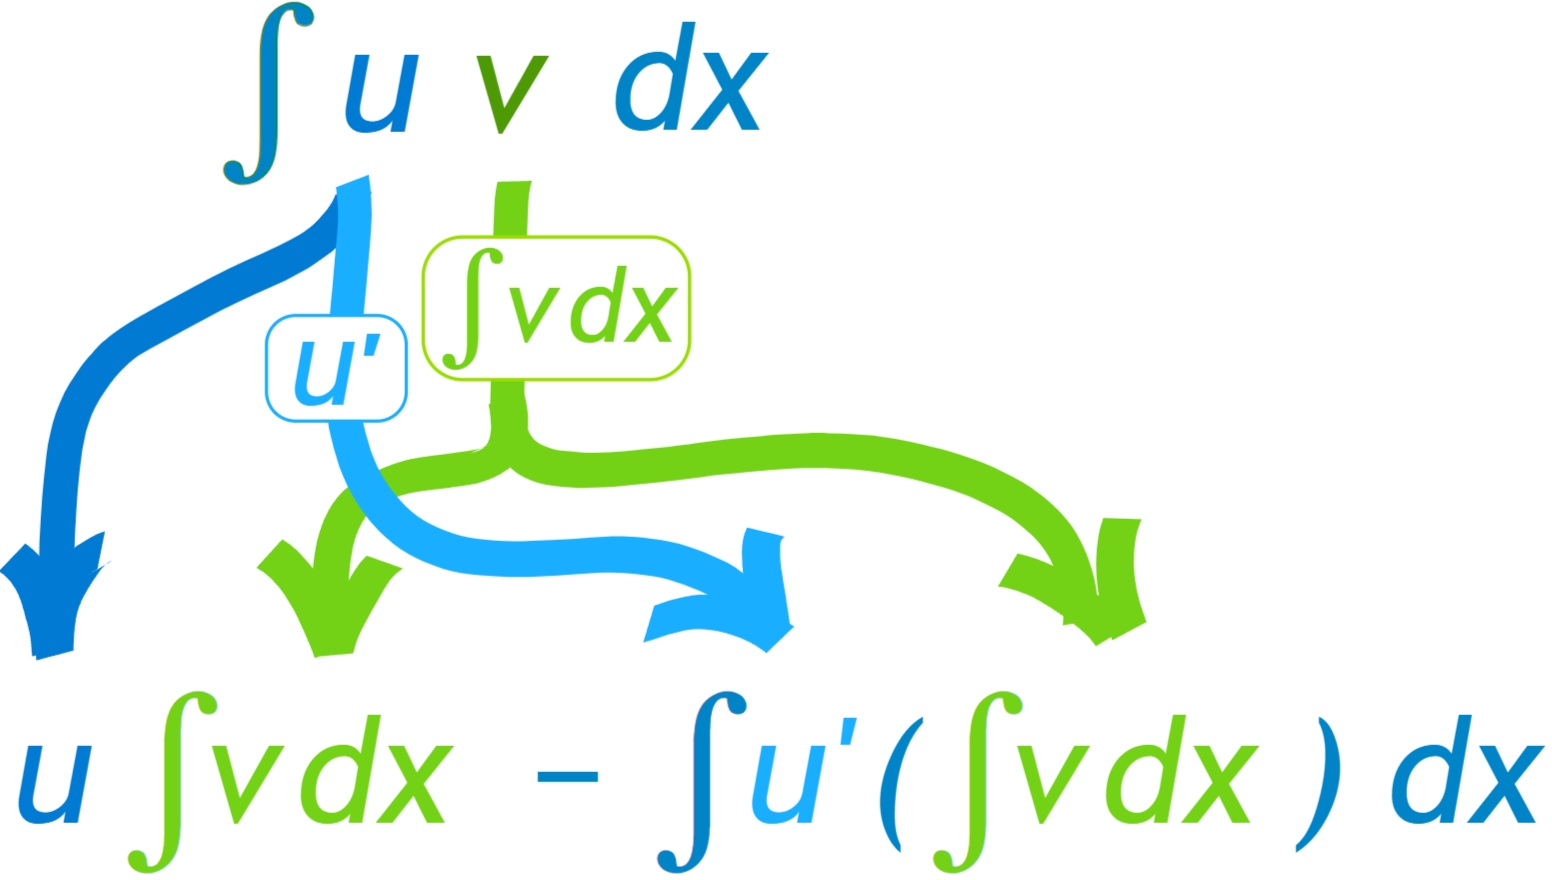
\includegraphics[width=0.5\linewidth]{math/15.png}
    \caption{Integration by parts diagram, courtesy of Math is Fun}
    \label{fig:m15}
\end{figure}

\textbf{Integration by substitution} or \textbf{the reverse chain rule} requires you to set up your chained function in a particular way. Assume:
\[
    g(x)=u
    \qquad
    g'(x) \;dx=du
\]
We can use $u$ as an input placeholder and compute our integral as:
\begin{equation}
    \int f(g(x) \cdot g'(x)) \;dx
    = \int f(u) \;du
\end{equation}
After that, solve the integral normally (remember the variable is now a placeholder $u$) before substituting $g(x)$ back into the equation. Use figure \ref{fig:m17} to assist you when setting up the equation.
\begin{figure}
    \centering
    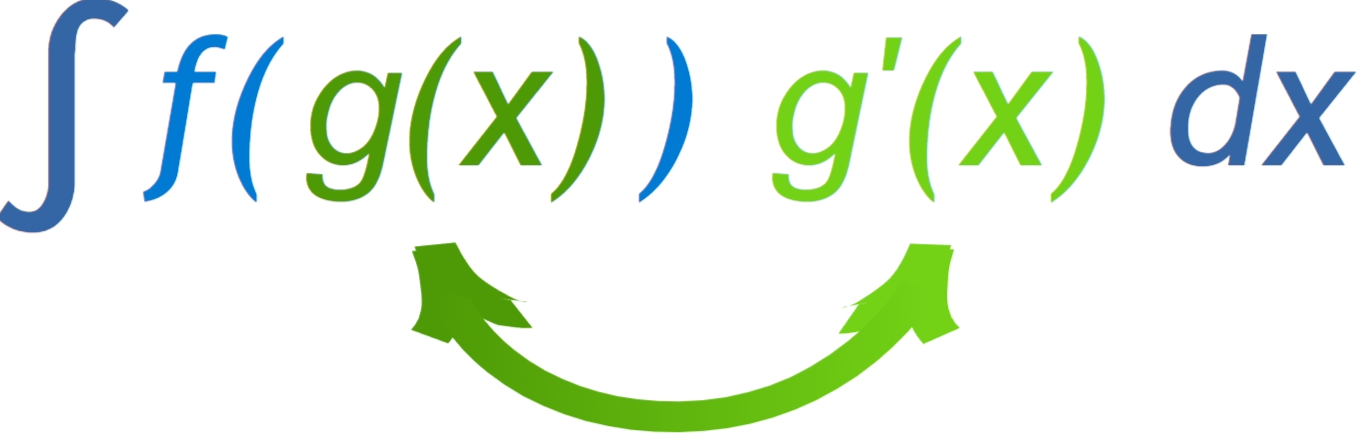
\includegraphics[width=0.4\linewidth]{math/17.png}
    \caption{Integration by substituting. courtesy of Math is Fun}
    \label{fig:m17}
\end{figure}

\subsection{The power rule}
The intuition has $nx^{n-1} = (x^n)'$ as the derivative's power rule. However, the left side is $n$ times larger than our function inside the integral. If we were to divide both sides by $n$, then the input would be the original function stated in the rule. Of course, the $n$ is offset by $1$ because we put it relative to the derivative on the right side.
\[
    nx^{n-1} = (x^n)'
    \Leftrightarrow x^{n-1} = \frac{(x^n)'}{n}
    \Rightarrow^{\text{-ish}} x^{n} = \frac{x^{n+1}}{n+1}
\]
Such a way of thinking will work, but as you can see, it is not accurate when you need to insert that "-ish" into the equation. As for the reason it is not accurate, did you realize that the final equation somehow dropped the derivative bracket?

\subsection{Integration by parts}
While it is true that we need to have $C$ for every integral result, it is not necessary in the case of the inner integrals $\int v\;dx$ because the $C$ will eventually cancel out.

It is important to identify which $u$ and $v$ to use to make the derivatives and integrals easier — you should choose a $u$ that gets simpler when you differentiate it and is similar to $v$ integration. A rule to remember is \textbf{I LATE}. You should choose $u$ based on which of these comes first:
\begin{itemize}
    \item \textbf{I}: inverse trigonometric functions such as $sin^{-1}$
    \item \textbf{L}: logarithmic functions like $\ln(x)$ or $log(x)$
    \item \textbf{A}: algebraic functions like $x^2$ or $x+1$
    \item \textbf{T}: trigonometric functions such as $\sin(x)$
    \item \textbf{E}: exponential functions such as $e^x$ or $3^x$ ($x$ as the power... you don't want to give something unknown the power)
\end{itemize}

\textbf{The formula} originates from algebra manipulation of the original product rule:
\[\begin{aligned}
    &(fg)' = fg'+f'g \\
    \Leftrightarrow& fg' = (fg)'-f'g \\
    \Leftrightarrow&\int fg'\;dx = \int(fg)'\;dx-\int f'g\;dx 
        &\text{Take the integral of every terms}\\
    \Leftrightarrow&\int fg'\;dx = fg -\int f'g\;dx
        &\text{Derivative cancels the integral}\\
\end{aligned}\]

\subsection{Integration by parts trick: the tabular method}
This is a quick trick to calculate the integral function that was set up according to our stated format $\int uv\;dx$ of the integration by parts rule. It is recommended that the reader find an online resource with videos to explain as it is much easier to understand with an interactive format. A recommended video was included in the additional material section \ref{sec:m-integral-material}.

It is best to show the procedure as an example. Let's say we have the following integral:
\[ \int x^3\sin x \;dx \]
We identify $u=x^3$ and $v=\sin x$. Next, we set up the table \ref{tab:m3}. For every row on the $u$ column, we take a derivative of the previous row; similarly, we take the antiderivative for every $v$ row. For the sign, you can either denote it on the arrow, make a separate column for it, or negate the results in the $u$ column; the last row of the sign column was left empty as a reminder that you will not take the last derivative into the final result.
\begin{table}
    \centering
    \begin{tabular}{|c|c|c|} \hline 
          Sign&$u$& $v$\\ \hline 
          $+$&$x^3$& $\sin x$\\ \hline 
          $-$&$3x^2$& $-\cos x$\\ \hline 
          $+$&$6x$& $-\sin x$\\ \hline 
          $-$&$6$& $\cos x$\\ \hline
          &$0$& $\sin x$\\ \hline
    \end{tabular}
    \caption{Example of the tabular method's table}
    \label{tab:m3}
\end{table}

Take a look at figure \ref{fig:m16} and now look at what one should get as a result. It is easier to remember the method visually than a wordy description.
\[\begin{aligned}
    \int x^3\sin x \;dx =
    &+ x^3 (-\cos x) \\
    &- 3x^2 (-\sin x) \\
    &+ 6x (\cos x) \\
    &- 6 (\sin x) \\
    =& -x^3\cos x + 3x^2\sin x + 6x\cos x - 6\sin x
\end{aligned}\]
\begin{figure}
    \centering
    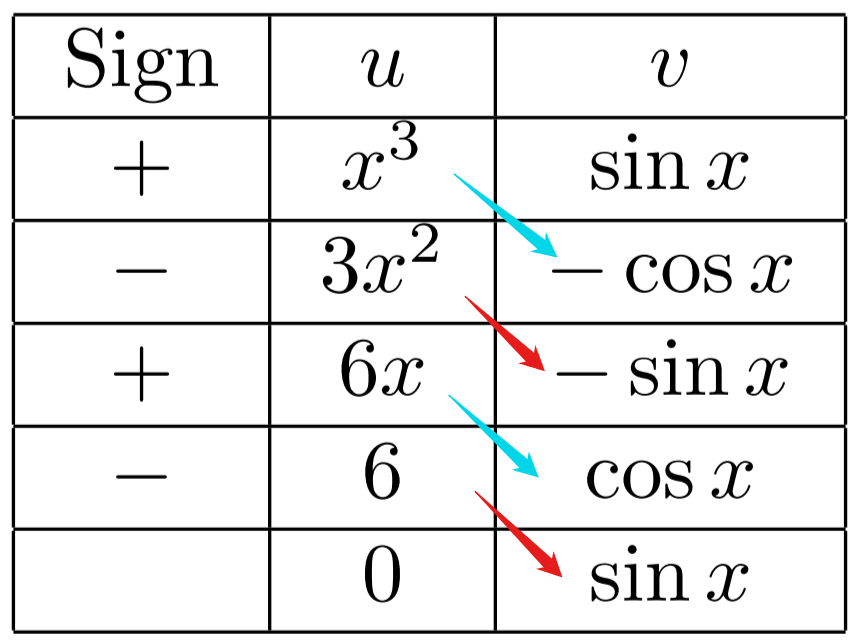
\includegraphics[width=0.4\linewidth]{math/16.png}
    \caption{Integration by part using the tabular method}
    \label{fig:m16}
\end{figure}

You need the $u$ column to eventually reach $0$ to make this method work. In case your table gets too long, maybe consider using the original integration by parts formula (\ref{eq:m5}). Furthermore, do not worry about accidentally going past the stop point, as the $0$ in the $u$ column should remind you that $a\times0=0$.

\subsection{Integration by substitution}
The listed formula somehow subtlety cancelled out everything but in reality, it is just simply an expansion of the derivative $du$ itself. Let's start fresh from an integral:
\[
    \int \cos(x^2) \cdot 2x \;dx
\]
We can define $u$:
\[
    u = x^2
\]
Therefore $u'$ or the derivative of $u$, notated with small changes in $du$ is:
\[
    \frac{du}{dx} = 2x
    \Leftrightarrow
    dx=\frac{du}{2x}
\]
Replace $dx$ into our integral, we can see the $2x$ were cancelled out nicely, making all the variables inside the integral become $u$ instead of $x$. After that, we can calculate the integral with our input variable as $u$, then substitute $u$ back to answer:
\[\begin{aligned}
    \int \cos(x^2) \cdot 2x \;dx
    &= \int \cos(u) \cdot 2x \;\frac{du}{2x} \\
    &= \int \cos(u) \;du \\
    &= \sin(u) + C \\
    &= \sin(x^2) + C
\end{aligned}\]

Note that most of the time, it is not possible to start with an already set-up function but it is okay: you can just go ahead and select a convenient $u$ and replace $dx=du/u'$. We have this example:
\[\begin{aligned}
    \int x\sqrt{x-1} \;dx
    &= \int x\sqrt{u} \;du
    \qquad\text{Define } u=x-1 \text{ and } du=dx \\
    &= \int (u+1)\sqrt{u} \;du
    \qquad\text{From the original definition: } x=u+1 \\
    &= \int (u+1)u^{\frac{1}{2}} \;du \\
    &= \int u^{\frac{3}{2}} + u^{\frac{1}{2}} \;du \\
    &= \frac{2}{5}u^{\frac{5}{2}} + \frac{2}{3}u^{\frac{3}{2}} \\
    &= \frac{2}{5}(x-1)^{\frac{5}{2}} + \frac{2}{3}(x-1)^{\frac{3}{2}}
    \qquad\text{Substitute } u=x-1 \\
    &= \frac{2}{5}\sqrt{(x-1)^5} + \frac{2}{3}\sqrt{(x-1)^3}
    \qquad\text{Add integration constant}
\end{aligned}\]

\section{Integral of common functions}
\textbf{The constant function} has a similar representation to the figure \ref{fig:m13} where the integral will increase the degree of a function. It is the power rule in equation (\ref{eq:m4}).
\begin{equation}
    \int a \;dx = ax + C
\end{equation}
If you continue to expand the power rule, we will have an integral for \textbf{linear function} and a \textbf{squared}:
\begin{equation}
    \int x \;dx = \frac{x^2}{2} + C
    \qquad
    \int x^2 \;dx = \frac{x^3}{3} + C
\end{equation}

\textbf{The reciprocal function} can be used for general situations or when $n=-1$ for the power rule:
\begin{equation}
    \int x^{-1} \;dx
    = \int \frac{1}{x} \;dx
    = \ln|x| + C
\end{equation}

\textbf{Exponential with Euler's number} is quite easy to remember if you remember that its derivative is always itself (with the $C$):
\begin{equation}
    \int e^x \;dx = e^x + C
\end{equation}

If we have \textbf{the variable as the power}, natural log once again came up:
\begin{equation}
    \int a^x \;dx = \frac{a^x}{ln(a)} + C
\end{equation}

And if we put \textbf{a natural log} on the table after appearing in so many equations, we have its integral as:
\begin{equation}
    \int \ln(x)dx
    = x \ln(x) - x + C
    % = x(\ln(x) - 1) + C
\end{equation}

\textbf{Trigonometric functions} can be remembered by recalling the original derivative trigonometric functions:
\begin{equation}
    \int \cos(x) dx = \sin(x) + C
    \qquad
    \int \sin(x) dx = -\cos(x) + C
    \qquad
    \int \sec^2(x) dx = \tan(x) + C
\end{equation}

\section{Additional material}\label{sec:m-integral-material}
\begin{itemize}
    \item A YouTube playlist by 3Blue1Brown to help with the visualization of constructing derivatives (as well as other calculus concepts): \href{https://www.youtube.com/playlist?list=PL0-GT3co4r2wlh6UHTUeQsrf3mlS2lk6x}{Essence of calculus}
    \item An in-depth look into the proof and connection between derivatives and integrals: \url{https://en.wikipedia.org/wiki/Fundamental_theorem_of_calculus}
    \item The tabular method explanation video: \url{https://www.youtube.com/watch?v=Yyic5aaXGaw}
    \item A strongly worded flowchart to solve integrals can be found in figure \ref{fig:m18}
\begin{figure}
    \centering
    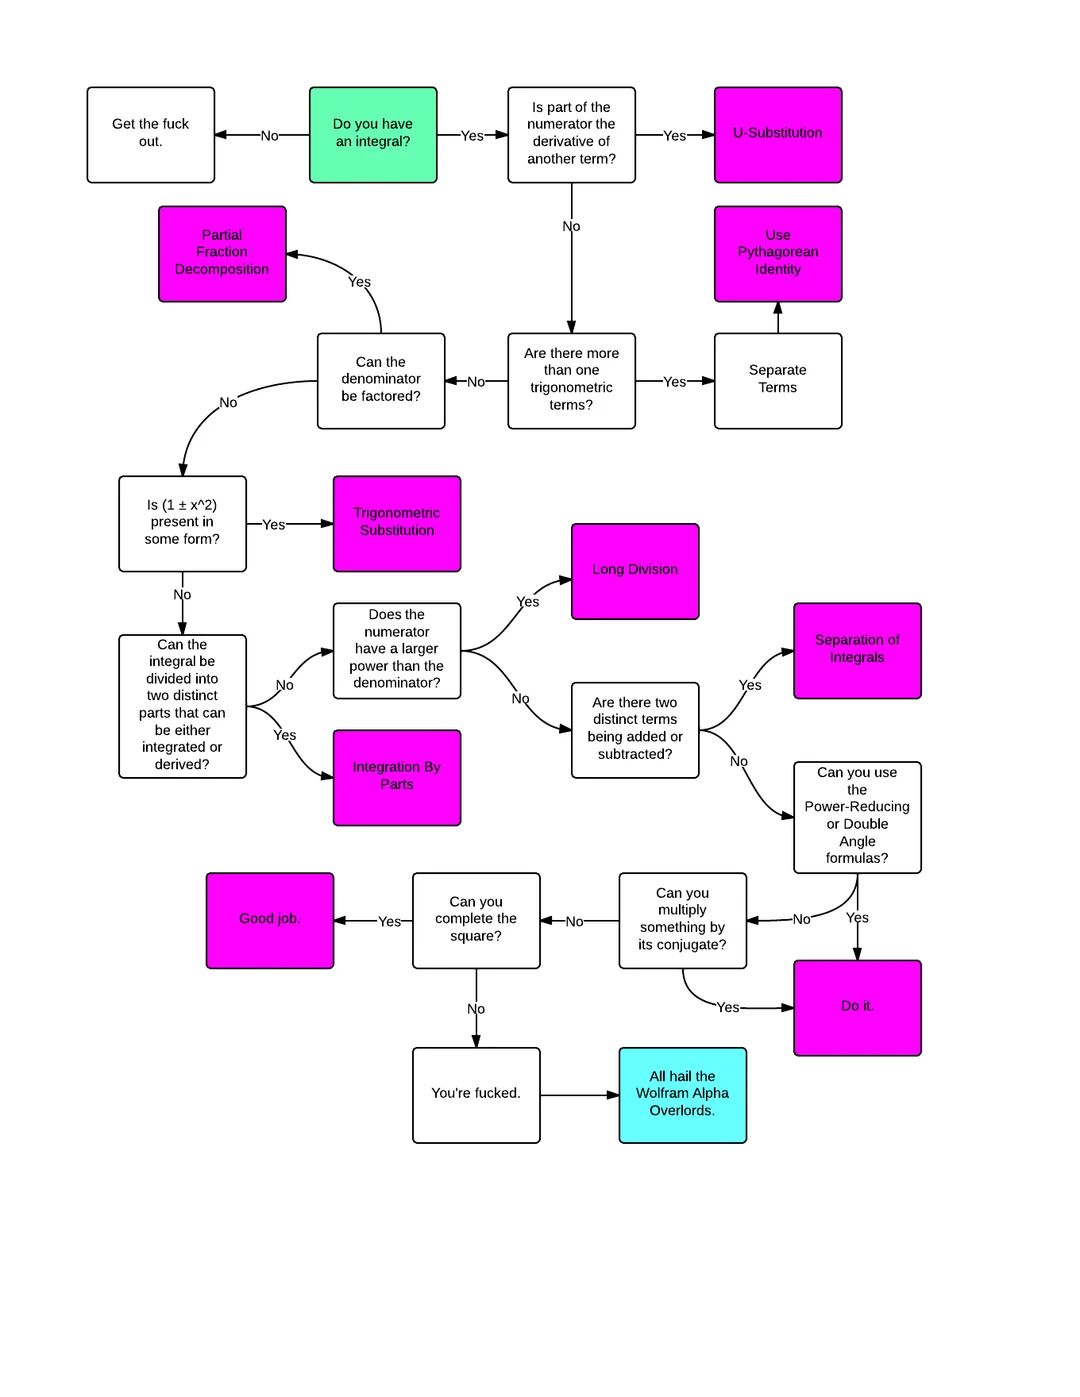
\includegraphics[width=1\linewidth]{math/18.png}
    \caption{Solving integrals flowchart, courtesy of a deleted Reddit user on r/math}
    \label{fig:m18}
\end{figure}
\end{itemize}